\chapter{Getting Real: the Challenge of Building and Validating a Large-Scale Digital Twin of Barcelona’s Traffic with Empirical Data\textsuperscript{*}}
\chaptermark{Getting Real: a Large-Scale Digital twin of Barcelona's traffic}
\label{ch:getting_real}
\graphicspath{{chapters/02_getting_real/figures/}}

\section*{Prologue: The city of pruning streets}
\addcontentsline{toc}{section}{Prologue: The city of pruning streets}
\footnotetext{* A version of this chapter has been published as a peer-reviewed article: \fullcite{ArgotaSanchez-Vaquerizo2021}. The prologue has been published as part of the book chapter: \fullcite{ArgotaSanchez-Vaquerizo2023_3Tales}.}

In this city, not every street is designed to make the circulation of vehicles easier, faster, and safer. When traffic jams happen, they do not build new roads \citep{Duranton2011}. They do just the opposite: they close roads or reduce the number of lanes. Over the years, the traffic in this city has not worsened, and the environmental quality of the streets has improved while making space for other activities and alternatives for mobility \citep{Rueda2018}.

People in this city rebelled against how things were decided before. First, they learned. They could not ignore the complex counterintuitive effects \citep{Braess1969,Roughgarden2005} of planning decisions made by experts around the world \citep{Cairns2002,Chung2012,Kolata1990}. Second, they changed citizens’ roles. They were not satisfied with simply being consulted about predefined plans designed by experts \citep{Blundell-Jones2005}. People wanted to be informed and participate, not be persuaded \citep{Cardullo2019}.

It took them some time to tune their city-making processes and combine the understanding of urban complexity with people’s desires and preferences to inform decisions in actionable, effective ways. Their planners became coordinators, facilitators, and systems designers and not mere makers of visionary prescriptions \citep{Ratti2015}. They leveraged the knowledge and goals of the various people and organizations involved in the wicked problem of designing their city \citep{Rittel1973} by expanding techniques of planning support systems \citep{Geertman2020} into hybrid human-machine simulations \citep{Licklider1960,Negroponte1970} with the support of artificial intelligence \citep{Lock2021}. They brought people into the loop. Everybody in this city can now experiment with their future simulated visions in such a way that they can reflect on and inform their opinions and images of their city \citep{Lynch1960} and let the computer intelligence learn to help them.

Planning in this city is a serious game \citep{Beirao2012,Dodig2019}. Its citizens, developers, investors, and designers, among other stakeholders, interact with highly accurate simulations of their environment in a safe sandbox. There, they explore alternatives, learn from the outcomes of their own actions, and sometimes adapt their opinions and preferences according to their experience \citep{Burr2018}. The use of artificial intelligence in this interactive decision-making system expands the capabilities of this city’s inhabitants to know, share, negotiate, and agree \citep{Engelbart1962}. They can communicate their preferences, aggregate them with fellow citizens, update possible scenarios, and hybridize them to offer new alternatives. More importantly, this system allows people’s opinions to be elaborated and coordinated in an actionable way. This framework is a collaborative development environment whose best versions are deployed for updating the real city as needed as if it were an operating system \citep{Marvin2017}.

In this creative generative loop, people experience and experiment through simulations of their desired city while the computer intelligence learns from them and helps to coordinate these human preferences in actionable ways to configure the new city \citep{Konig2017}. In a sense, it is much closer to a continuous, augmented, collaborative, and AI-mediated, even generative, dev-ops scheme with many humans-in-the-loop \citep{Chirkin2016,Scott2002,Veloso2021}. This city’s people have replaced their previous rigid and static planning with new dynamic city operations based on hundreds of cities simulated and wished for by humans in almost real time. Nowadays, they can adapt to the very rapidly changing conditions of their world, hit by overheated extreme weather and unstable ecosystems. What is more impressive, they can maximize their strategies with minimal intervention. They get more done by doing less.

\setcounter{figure}{-1}
\begin{figure}[htbp!]
    \centering
    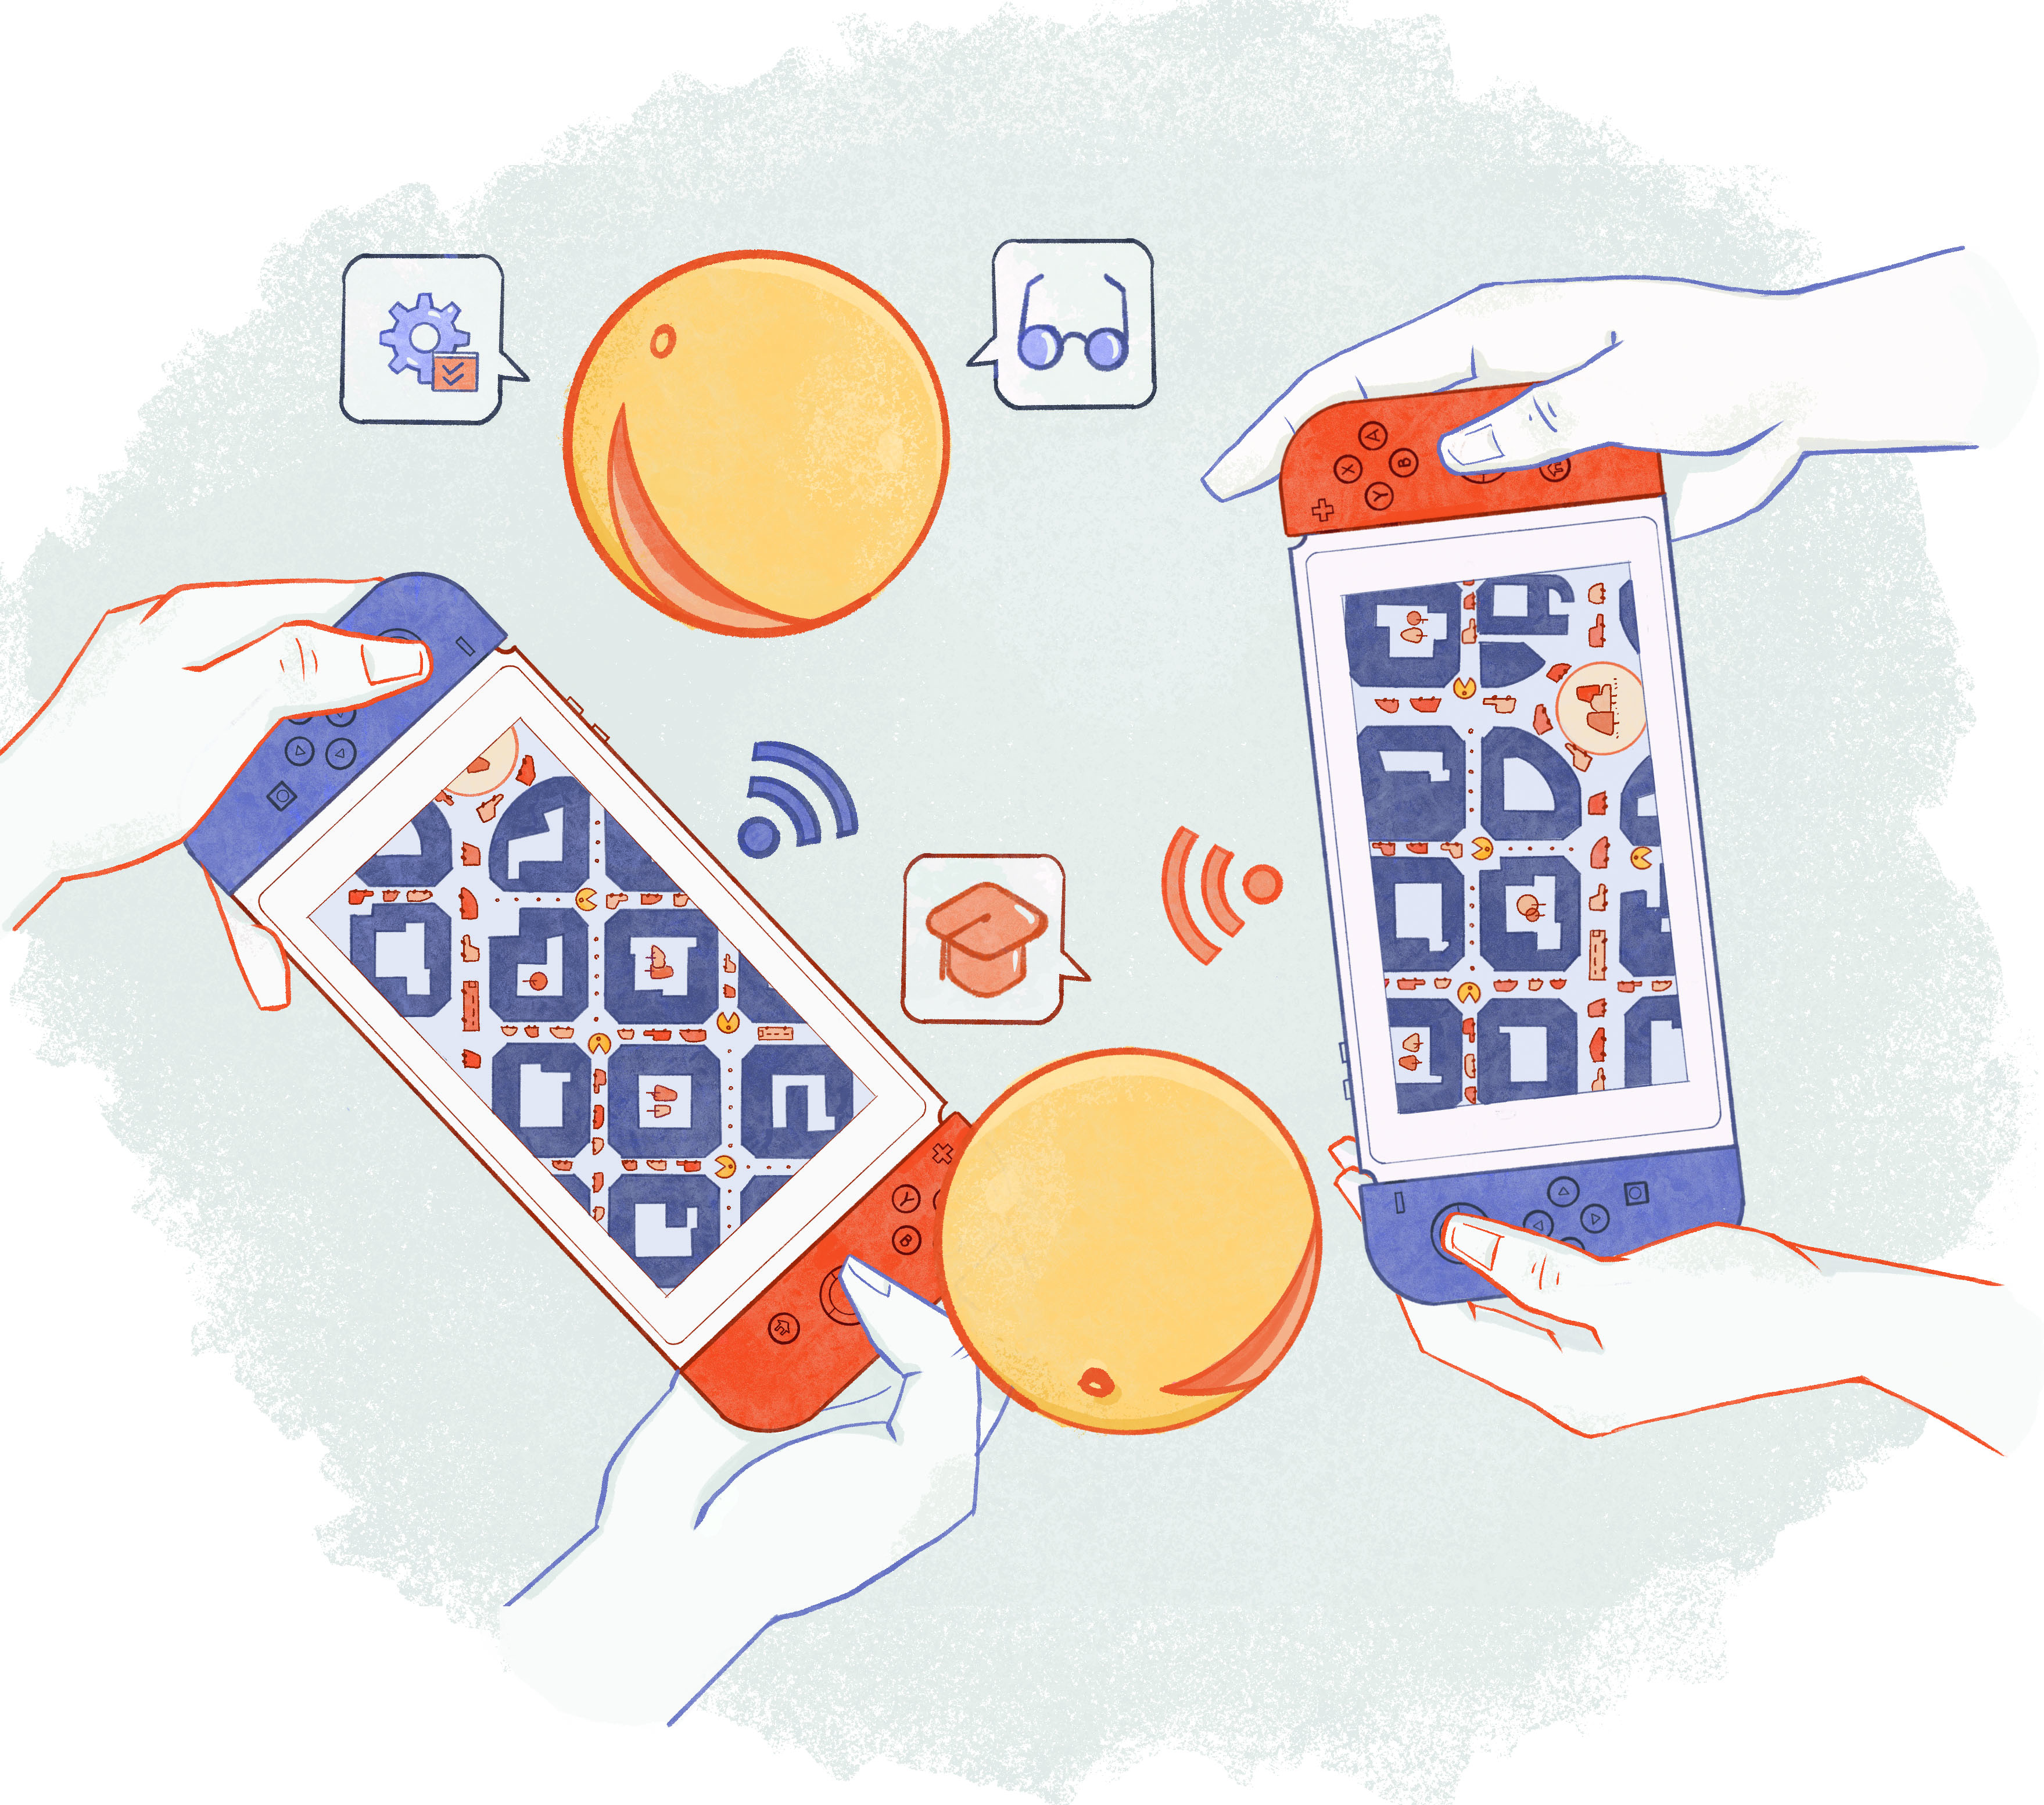
\includegraphics[width=1\textwidth]{chapters/02_getting_real/figures/fig_03_computer_intelligence.jpg}
    \captionsetup{format=plain, justification=centering} % Center the caption
    \caption{Computer intelligence pairs with people and enhances communication and coordination.}
   \label{fig:hybrid_intelligence}
\end{figure}
\FloatBarrier

\section*{}
\chapterabstract{
Large-scale microsimulations are increasingly resourceful tools for analysing in detail citywide effects and alternative scenarios of our policy decisions, approximating the ideal of ‘urban digital twins’. Yet, these models are costly and impractical, and there are surprisingly few published examples robustly validated with empirical data. This paper, therefore, presents a new large-scale agent-based traffic microsimulation for the Barcelona urban area using SUMO to show the possibilities and challenges of building these scenarios based on novel fine-grained empirical big data. It combines novel mobility data from real cell phone records with conventional surveys to calibrate the model comparing two different dynamic assignment methods for getting an operationally realistic and efficient simulation. Including through traffic and the use of a stochastic adaptive routing approach results in a larger 24-hour model closer to reality. Based on an extensive multi-scalar evaluation including traffic counts, hourly distribution of trips, and macroscopic metrics, this model expands and outperforms previous large-scale scenarios, which provides new operational opportunities in city co-creation and policy. The novelty of this work relies on the effective modelling approach using newly available data and the realistic robust evaluation. This allows the identification of the fundamental challenges of simulation to accurately capture real-world dynamical systems and to their predictive power at a large scale, even when fed by big data, as envisioned by the digital twin concept applied to smart cities.}

\section{Introduction}

Cities are complex systems \citep{Port00} that feature non-stationary behaviour \citep{Gershenson2013}, that is, they are in constant change and transformation. To increase the quality and resilience of urban areas, new forms of mobility, together with different patterns of (land) use, and a redesign of spaces are proposed, which are typically characterized by as much chaos as order. This makes them unsuitable for traditional control approaches, as the involved conditions and problems are always evolving. This complexity of urban settings makes it particularly difficult to assess and evaluate the feedback, side and cascading effects of policies, decisions, and behaviours. Unfortunately, testing in real-life settings is costly, risky, sometimes unethical, and often unfeasible. Even in the case of piloting, the possibility of extrapolating and scaling results is questionable.

Alternatively, it is possible to develop computer-based simulation models that try to capture the functioning of a city as accurately as possible \citep{Batty2018}. The development of such virtual scenarios allows testing, assessing, and measuring the impact of change at reduced cost and risk, with higher flexibility, and a capacity to control the conditions better than possible in real life. These so-called digital twins \citep{Grieves2014} are fed with (partly real-time) smart city data \citep{White2021} and are the goal of many cities \citep{Schrotter2020,AyuntamientodeMadrid2021,GovernmentofSingapore2018,EuropeanCommission2019,Airaksinen2019,Hourdos2008}, thereby pushing the long tradition of urban simulation \citep{Lowry1964,Forrester1969,Acheampong2015,Wegener2021Land-UseModels} to the technological cutting edge. The progressive spread of cyber-physical systems \citep{Tomko2019,Batty2019} becomes a powerful opportunity for real-time management, for anticipating possible outcomes of planning and policy decisions before implementations are made, and for fostering co-creation and citizen participation \citep{White2021}.

However, many of the envisioned changes are on a small and high-frequency scale \citep{Batty2018,Wildfire2018}. That is, on the scale of people’s perception and experiences, such as drivers getting around, new forms of mobility, the spatial configuration of buildings, streets, and public spaces, the design of infrastructures, and the emergence of new smart digitally-enabled systems. Therefore, the use of simulations as planning tools needs the high level of interpretability and detail obtained by microsimulations capabilities \citep{Treiber2013}. Despite all the incremental details, depth, and richness of information becoming available, it is needed to account for necessary simplification \citep{Batty2018}, non-measurable qualities, as well as limitations and uncertainties when it comes to the behaviour of people and socio-cultural systems, which need to be included \citep{Mathias2020}.

Therefore, the challenge is to build and validate realistically a microsimulation of a large urban area, to study on a small scale of detail citywide policies. This paper presents a pipeline to build a digital twin for the traffic flow in the large, dense, and congested urban area of Barcelona, Spain, based on novel cell-phone mobility data and publicly available databases using the SUMO agent-based microsimulation framework \citep{Lopez2018}. The paper is organised as follows. \autoref{subsec:GR_1.1_existing_large_scale_micro} introduces existing large-scale urban microsimulation scenarios. \autoref{sec:GR_2_mats_and_meths} describes the pipeline to build the proposed model, including the pre-calibration of parameters. \autoref{sec:GR_3_val} explains the evaluation of the results of the simulation scenarios based on a robust multi-variable comparison with real measured data, namely with respect to various metrics on different spatio-temporal scales. Finally, \autoref{sec:GR_4_dis} expands on limitations, possible applications, and potential future research.


\subsection{Existing Large-Scale Urban Microsimulation Scenarios}
\label{subsec:GR_1.1_existing_large_scale_micro}

Agent-based microsimulations follow the logic that larger-scale effects observed in the physical reality can be obtained by the aggregation of emulated individual properties and behaviours of agents at a small scale (such as the individual position, speed, and acceleration) \citep{Helbing2010}. However, they require large amounts of detailed disaggregated data and long processing times, needing considerable computational resources both for calibrating and for running them. Determining the many parameters describing individual behaviours and the interactions of numerous agents, are among the main challenges in building, calibrating, and evaluating these models. This results in compromises in terms of realism, while one needs to consider that minor errors in any of these components may propagate and cumulate, thereby producing deviations or even incorrect results \citep{Heppenstall2012}.

The relatively few published examples of complete, comprehensive, and validated large-scale urban scenarios using microsimulations reflect this complexity. Urban settings are even more challenging to calibrate and build than equivalent interurban settings \citep{Kastner2014,Urquiza-Aguiar2019}, because of very high levels of mobility demand concentrated in small areas with complex, dense, and intricate networks.

The numerous examples of building, calibrating, and validating traffic simulations in scientific literature and policymaking \citep{Hourdos2008,Balakrishna2007,Oketch2005,Bartin2018,Rodriguez-Rey2021,Bassolas2019} show this complexity trade-off between size and level of detail: large-scale models are more suitable for macro and mesoscopic approaches, while detailed microsimulations focus on smaller scenarios \citep{Saidallah2016}. This bounds their operational possibilities and limits the detailed study of citywide interventions and policies \citep{Hardy2008}. Precisely, this paper focuses on this gap in the urban simulation literature: the lack of large-scale urban scenarios that use traffic microsimulation \citep{McKenney2013,Soares2014,Bieker2015}, and missing robustly quantitative validation with real data \citep{McKenney2013,Uppoor2011,Codeca2018,Rapelli2019,Behrisch2019,Gueriau2020,PereiraMachado2020} (see \autoref{tab:large_scale_traffic_simulation_examples}). Reviewing the few scenarios combining a large-scale scope with a microscopic approach supports the design of the proposed new data pipeline for building, calibrating, and validating the model while being able to highlight and address the existing challenges:

\begin{itemize}
    \item Large urban microscopic scenarios are complicated and slow, which obstructs microsimulation over extended periods of time, as well as their calibration (requiring multiple runs with different parameter sets);
    \item This causes compromises between efficiency and realism;
    \item Validation is often based on a qualitative assessment of results or lacks a quantitative comparison with empirical measurements (requiring a different data set than used for calibration);
    \item The empirical data needed are frequently incomplete or inaccurate.
\end{itemize}

However, beyond the different combinations of data sources and strategies for demand creation used by these urban simulations, their most relevant differences are in their size and validation methods. The lack of commonly established approaches and the differences in available observational data in each location for validation makes it difficult to assess the results and consequently to compare them regarding size, duration, and realism.
Therefore, this paper analyzes existing examples to develop further large-scale microscopic urban simulations with a wide multi-scalar realistic validation supported by observational data. It aims to provide a feasible path to investigate their new operational capabilities and limitations, both in applicability and developments steps within the increasing interest of the so-called ‘digital twins’.

Hence, the proposed microsimulation for the large urban area of Barcelona combines novel mobility data from cell phone records and publicly traditional surveys with detailed urban network data extracted from OpenStreetMap. The quantitative validation is based on a different empirical data set over 24 h using various metrics. As a result, reportedly, this model is one of the most complete published large-scale urban traffic microsimulations regarding the scope, network size, duration, and realism (validation). Hence, this is probably the most detailed simulation scenario based on continuous-in-time car-following and route choice models currently known, which allows us to judge the potentials, challenges, and limitations of the “digital twin” approach including the technical feasibility of the concept, its safety, societal impact, and predictability power (see \autoref{sec:GR_4_dis}).

\section{Materials and Methods: Building of the Scenario}
\label{sec:GR_2_mats_and_meths}

The construction of a new microsimulation model for the urban area of Barcelona is based on the use of traditional data sources, including publicly available geographical information and conventional surveys, as well as new big data, specifically anonymized mobility data from mobile phones geographic position records. The general pipeline (\autoref{fig:getting_real_01_diagram}) shows the three main steps for building the scenario. The first step involves the generation of the transport system network and the travel demand. In the second step, the travel demand is adapted to find an efficient spatial distribution of routes through microsimulations. Finally, the third step compares the results of the resulting microsimulations from stage two with real-world data to evaluate how well the model fits the empirical ground truth.

The microsimulation software SUMO \citep{Lopez2018} is particularly suited for this purpose because of its open-source design, offering microscopic and mesoscopic capabilities able to conveniently provide detailed descriptions of interactions \citep{Treiber2013} and great versatility for scenario building \citep{Diallo2021,Urquiza-Aguiar2020}. Among others, it supports different data formats, demand modelling based on synthetic and real populations, different assignment approaches and route choice methods \citep{Gawron1998,GermanAerospaceCenterDLRandothers2021e}, as well as routing algorithms \citep{Dijkstra1959,Hart1968,Geisberger2008}.

The construction of an urban model to simulate mobility patterns requires two basic components: (i) a network, as the virtual environment where the agents will move, and (ii) a demand pattern that will generate the flows between the different locations of the mentioned network. In this case, the focus of the study is on the interaction between the (public) road infrastructure and the (private) vehicle traffic. Over here, public transportation and freight flows (~5\% of traffic flow) are not taken into account.

\begin{figure}[htbp!]
    \centering
    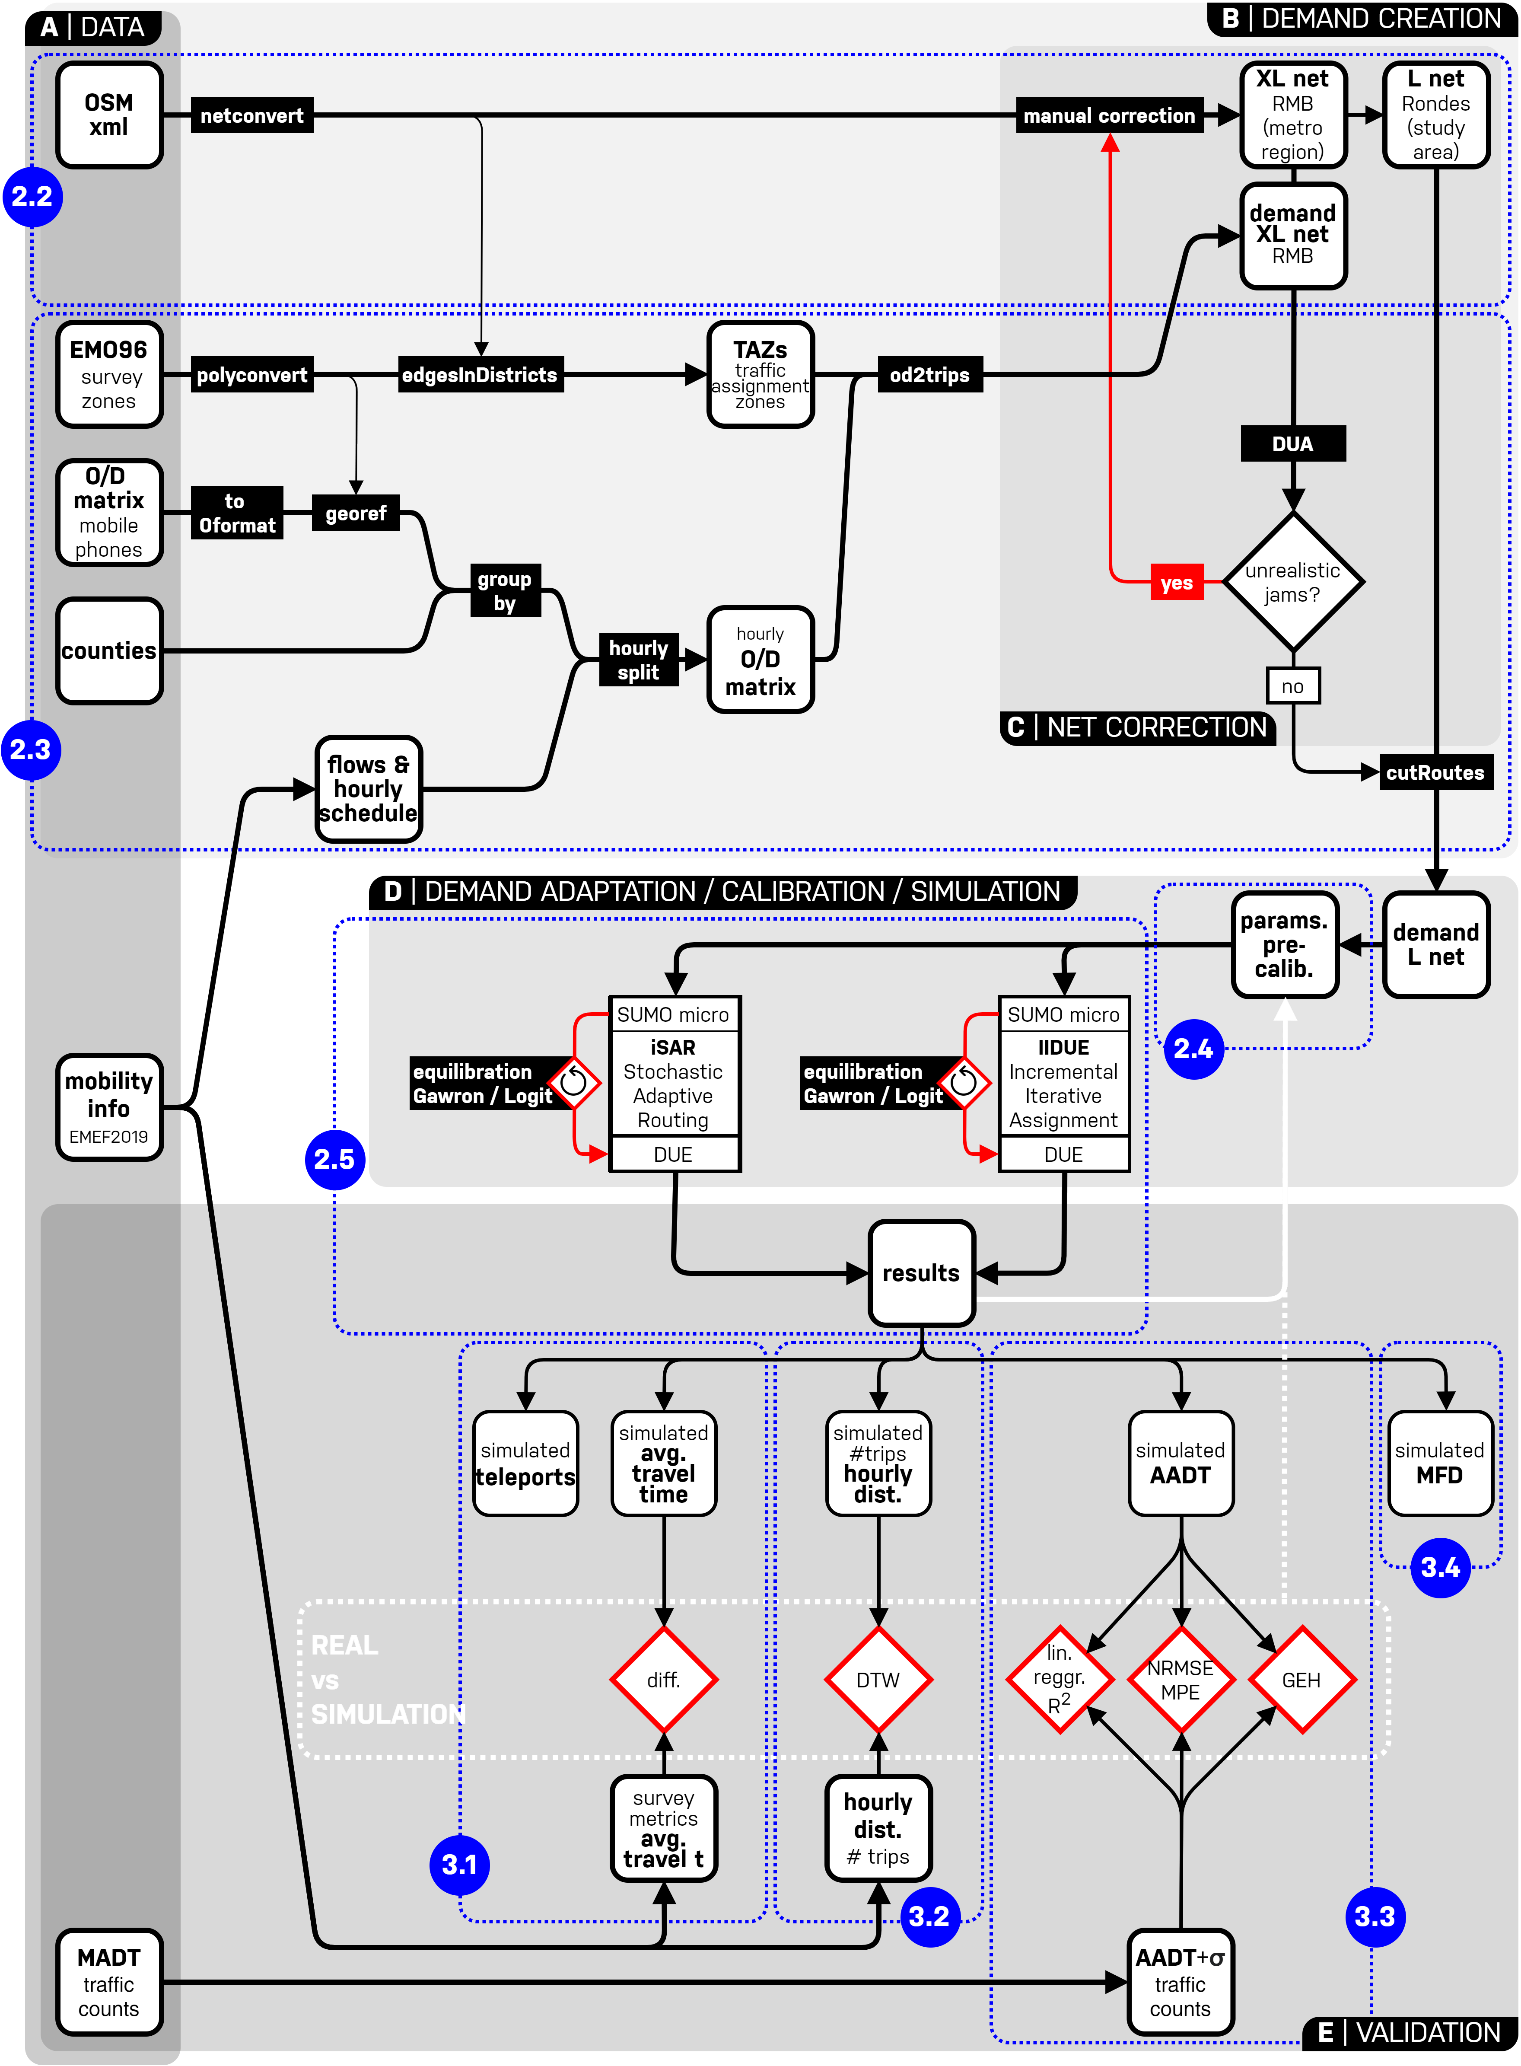
\includegraphics[width=1\textwidth]{fig_01.png}
    % \captionsetup{format=plain, justification=centering} % Center the caption
    \caption{Proposed data pipeline to build the microsimulation scenario. In blue, the sections of this paper are referenced.}
   \label{fig:getting_real_01_diagram}
\end{figure}
% \FloatBarrier

\subsection{Geographic Scope}

The implementation of the microsimulation model covers more than the city of Barcelona itself (Figure 2). The selection of the Metropolitan Region of Barcelona (\emph{Regió Metropolitana de Barcelona} or RMB) as the extended initial area of the model, larger than the city itself, allows including the relevant through traffic for the core area. The RMB has a size of 3126 km2 and contains about 5,103,000 inhabitants (~40\% of the surface and ~90\% of the population of the province of Barcelona). It includes the counties (\emph{comarques}) of Alt Penedès, Baix Llobregat, Barcelonès, Garraf, Maresme, Vallès Occidental, and Vallès Oriental. Additionally, surveys use alternative zoning for mobility statistics, based on concentric metropolitan subareas or belts (city of Barcelona, rest of the inner Metropolitan Area, outer Metropolitan Area, and rest of the RMB) (\autoref{fig:getting_real_02_geo_scope}a). Altogether, the vehicular trips between Barcelona and any of the locations within the RMB represent 96\% of all the daily car trips measured in the city (i.e., less than 4\% of car trips within the city limits of Barcelona are related to locations out of the RMB) \citep{InstitutdEstudisRegionalsiMetropolitansdeBarcelonaIERMB2020} (\autoref{tab:main_metro_domains}).

Thus, this expanded spatial scope allows capturing the complete traffic demand in the denser part of the urban area of Barcelona. Differently than in previously published microsimulation scenarios, where the network size and complexity in extended urban regions are frequently cropped or topologically simplified \citep{Tilg2020,Schweizer2021}, in this research, the extended metropolitan region (RMB) is initially simulated with full detail to provide the complete spatial distribution of trips within the core area. This core area (see \autoref{fig:getting_real_02_geo_scope}b) is not based on administrative divisions but on the functional and typological characterization defined by the main ring roads of the city (i.e., \emph{Ronda Dalt} and \emph{Ronda Litoral}, hence its name, Rondes). It includes the built-up area of the city of Barcelona and parts of a few surrounding municipalities (l’Hospitalet de Llobregat, Cornellà de Llobregat, Esplugues de Llobregat, el Prat de Llobregat, Sant Adrià de Besòs, Santa Coloma de Gramenet, and Moncada i Reixac). This compromise between realism and simplification allows preserving a realistic representation of the whole traffic demand of a very large urban area without simplifications while keeping the complexity of the network reasonably well by focusing on the part of the urban area that suffers the highest levels of congestion (i.e., Rondes).

\begin{figure}[htbp!]
    \centering
    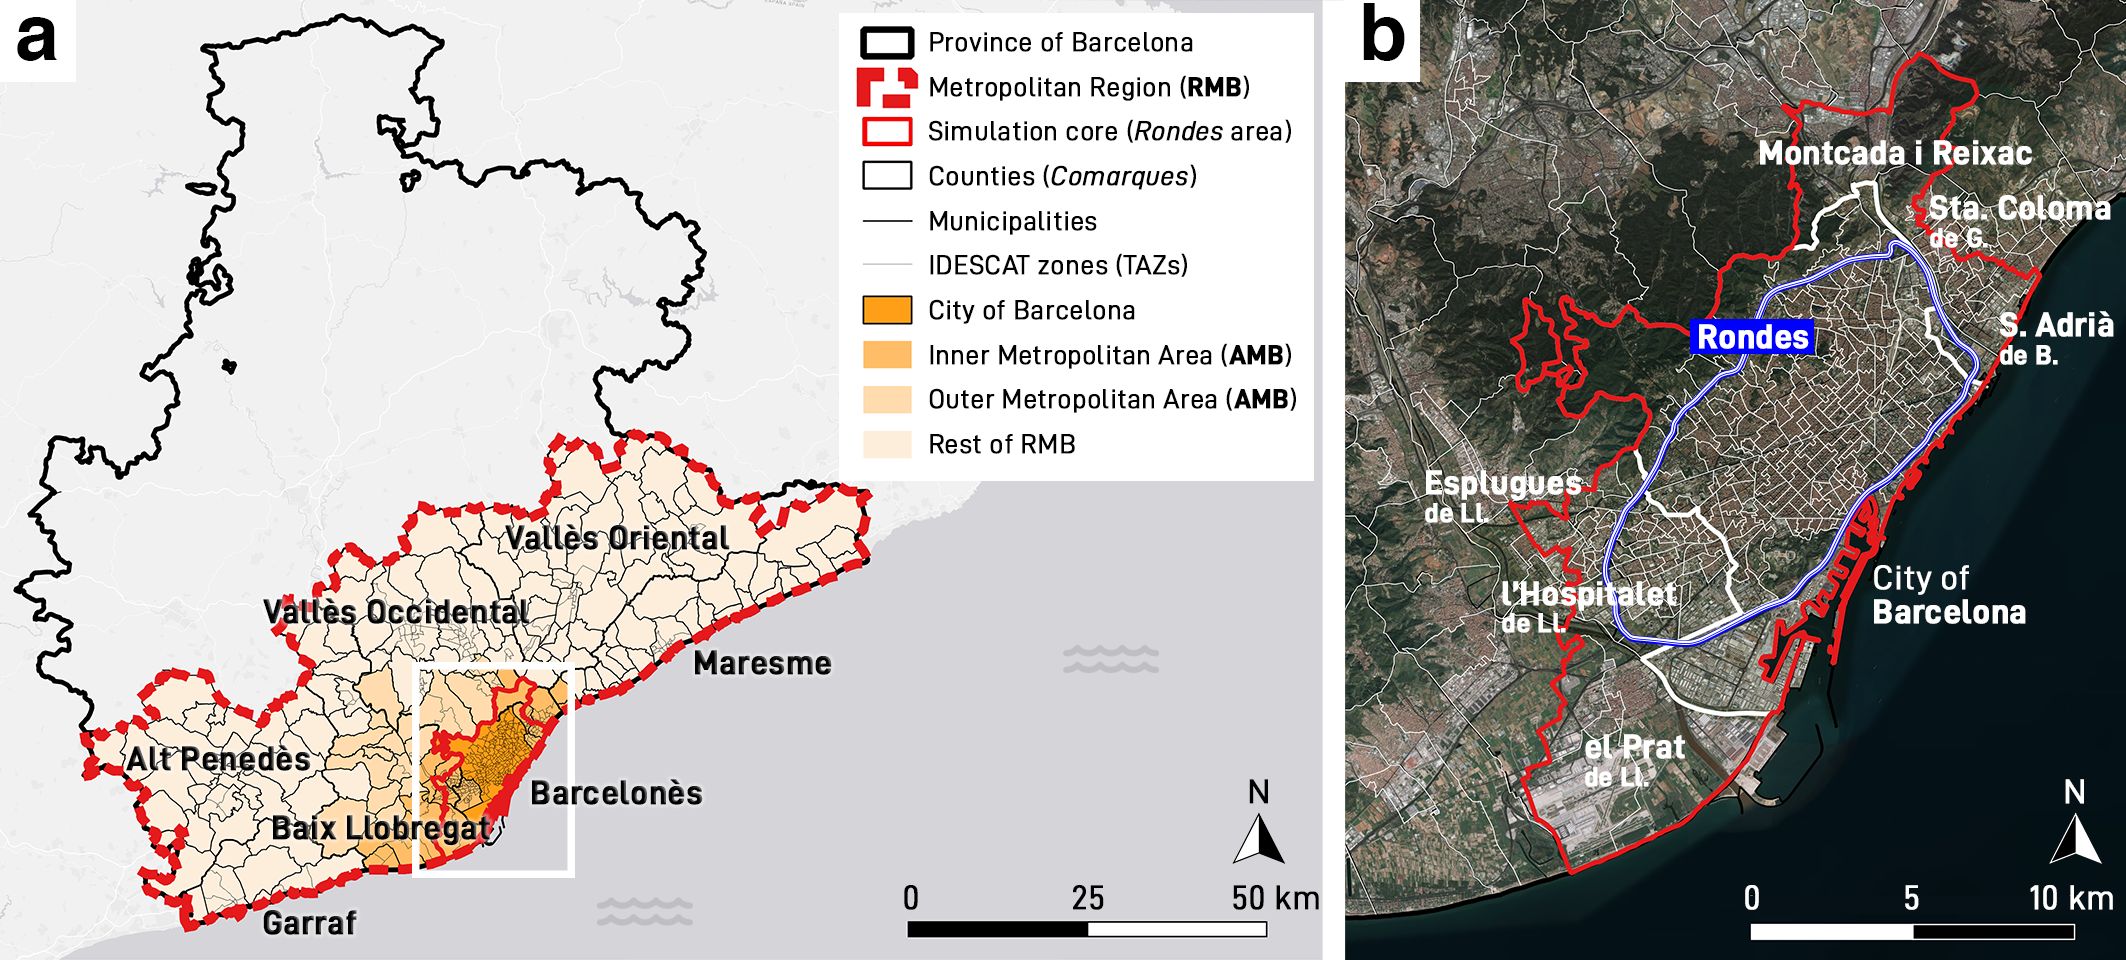
\includegraphics[width=1\textwidth]{fig_02.png}
    % \captionsetup{format=plain, justification=centering} % Center the caption
    \caption{Geographical domains covered by the microsimulation: (\textbf{a}) Location of the RMB within the province of Barcelona, including the different geographical divisions used in the model; (\textbf{b}) Core area of the detailed microsimulation (in red) defined by the city ring roads (Rondes, in blue) and corresponding Traffic Assignment Zones (TAZs, in white).}
   \label{fig:getting_real_02_geo_scope}
\end{figure}

% \usepackage{graphicx}
% \usepackage{booktabs}
% \usepackage{colortbl}


\begin{table}[hb!]
\centering
\caption{Characterization of main metropolitan domains.}
\label{tab:main_metro_domains}
\arrayrulecolor{black}
\resizebox{\linewidth}{!}{%
\begin{tabular}{lcccc} 
\toprule
\textbf{~}                & \begin{tabular}[c]{@{}c@{}}\textbf{Province of }\\\textbf{Barcelona}\end{tabular} & \begin{tabular}[c]{@{}c@{}}\textbf{RMB }\\\textbf{ (Extended area)}\end{tabular} & \begin{tabular}[c]{@{}c@{}}\textbf{\textit{Rondes} area }\\\textbf{ (Simulation Core)}\end{tabular} & \begin{tabular}[c]{@{}c@{}}\textbf{City of }\\\textbf{ Barcelona}\end{tabular}  \\ 
\hline
Area (km\textsuperscript{2})                & 7,726                                                                             & 3,126.2                                                                          & 182.55                                                                                              & 101.35                                                                          \\
Population (2019)         & 5,664,579                                                                         & 5,151,263                                                                        & 2,411,755                                                                                           & 1,636,762                                                                       \\
Total trips (any mode)    & 19,259,471                                                                        & 17,430,628                                                                       & 8,176,511                                                                                           & 5,682,214                                                                       \\
Trips in private vehicles & 6,946,355                                                                         & 5,927,332                                                                        & 2,063,177                                                                                           & 1,653,183                                                                       \\
\bottomrule
\end{tabular}
}
\arrayrulecolor{black}
\end{table}

\subsection{Transport Network}

For the creation of the urban network, the use of collaborative platforms offers open-source geographical data with a high degree of precision. OpenStreetMap (OSM) \citep{Haklay2008} is probably not only the best-known example of volunteered geographic information (VGI) \citep{Haklay2010}, it is also used by corporations as a mapping alternative to technologies such as Google Maps \citep{Anderson2019}. Additionally, SUMO provides convenient tools to transform OSM data into networks suitable for microsimulations.

Given the large area to be modelled, a script based on OSMNX \citep{Boeing2017} is adapted for downloading OpenStreetMap data \citep{OpenStreetMap} in XML format using the Overpass API \citep{wiki:xxx}, preserving all the relevant features for a microsimulation, including access and turning restrictions, speed limits, priority and class of roads, directions of circulation, traffic signs, and the number of lanes. SUMO’s \emph{netconvert} tool \citep{GermanAerospaceCenterDLRandothers2021d}, allows transforming this OSM XML file into an appropriate directed road network that encodes all the relevant features in the SUMO network format. This process relies on a good number of heuristics that try to translate the original OSM attributes into connectivity features, particularly regarding the layout of intersections, rights of access, and the positioning and coordination of traffic lights settings.

Note that the frequently inconsistent quality of OSM data \citep{Haklay2010} directly affects the creation of the network \citep{Dingil2018}. Misspecifications in mapping features such as intersections layout, number of lanes, speed limits, or traffic restrictions lead to unrealistic simulation outcomes that can considerably affect the performance of the model, for example, a lower traffic throughput (see \autoref{fig:getting_real_03_OSM_process}).

\begin{figure}[htbp!]
    \centering
    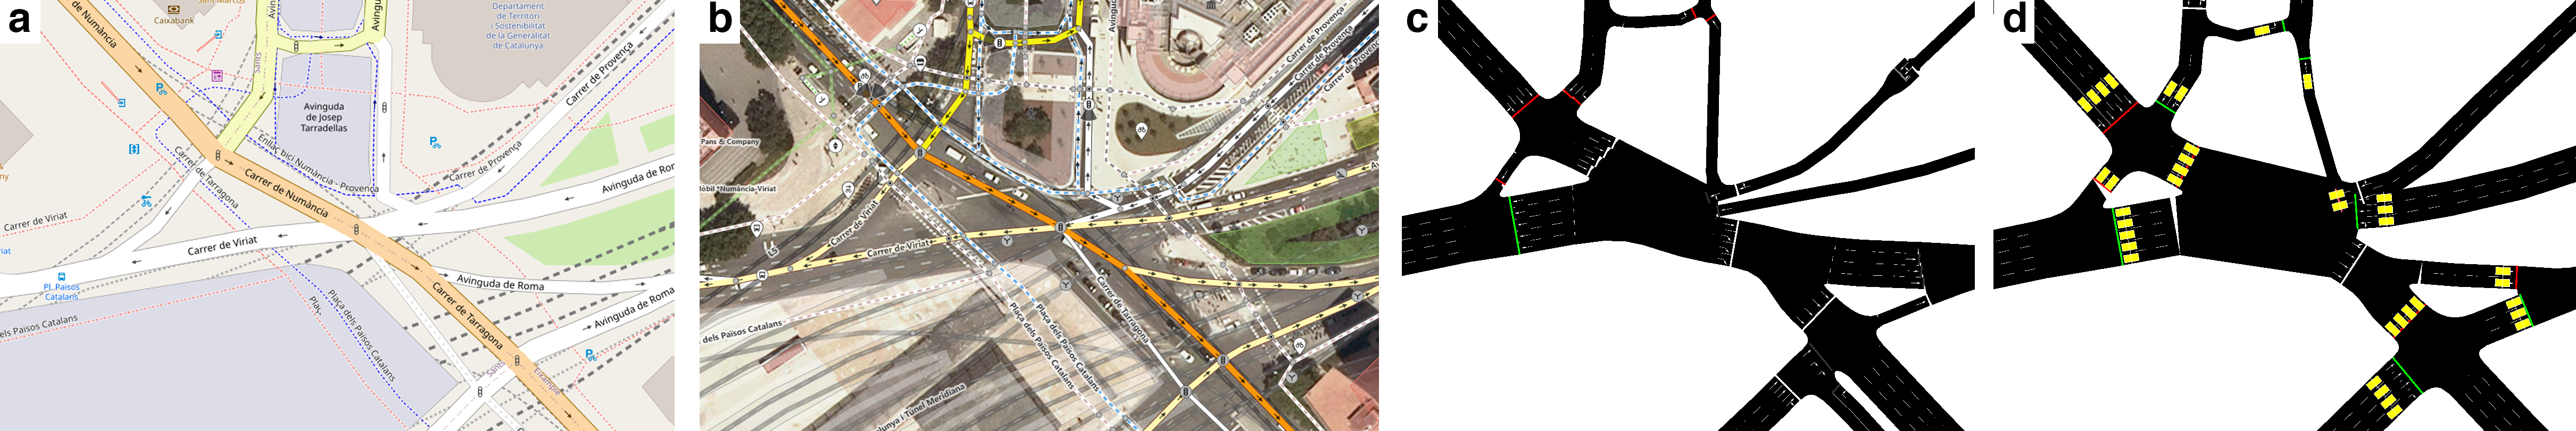
\includegraphics[width=1\textwidth]{fig_03.png}
    % \captionsetup{format=plain, justification=centering} % Center the caption
    \caption{Process of OSM data acquisition and edit for network generation: (\textbf{a}) OSM data; (\textbf{b}) OSM data correction based on third-party satellite imagery; (\textbf{c}) SUMO network with conversion errors (e.g., misspecifications of the lanes number, traffic lights, etc.); (\textbf{d}) final corrected SUMO network used for the simulation including virtual induction loops to measure traffic flows.}
   \label{fig:getting_real_03_OSM_process}
\end{figure}

To prioritize the vast task of correcting the large road network, whether due to errors caused by mapping misspecifications, wrong outcomes of SUMO conversion heuristics, or a combination of both, two complementary approaches are applied:
\begin{itemize}
    \item Short simulation runs using direct assignments of the traffic demand are employed to identify major errors hindering traffic performance.
    \item Satellite [60–63]\citep{Maxar2021,InstitutoGeograficoNacionaldeEspanaIGN2018,Sources:Esri2021,Sources:NASA2021} and street-level [64,65]\citep{GrabHoldings2021,Mapillaryandcontributors2021} imagery are used as independent third-party reference (ground truth) for correction.
\end{itemize}

Most of the needed corrections were done directly on OSM servers, contributing to the collaborative aim of the platform, by improving and updating the quality of the map in the area. Some fine-tuning has been performed directly in the definitive SUMO net file, using SUMO’s \emph{netedit} tool \citep{GermanAerospaceCenterDLRandothers2021c}, correcting errors caused by \emph{netconvert}’s conversion heuristics, particularly regarding intersections and traffic lights. Traffic light plans are a very relevant feature. In the current model, the real traffic light system used by the city was not available to us and, hence, not utilized. To simulate a realistic, simple, and efficient management of regulated intersections, the \emph{actuated} option of SUMO is chosen for all the traffic lights plans \citep{Koonce2008}. As a result, the network in the extended simulated area (RMB) covers a mix of urban, suburban, and rural areas. Differently, the core area (Rondes) has a very urban and dense character  (\autoref{fig:getting_real_04_road_net} and \autoref{tab:road_nets} for networks details).

\begin{figure}[htbp!]
    \centering
    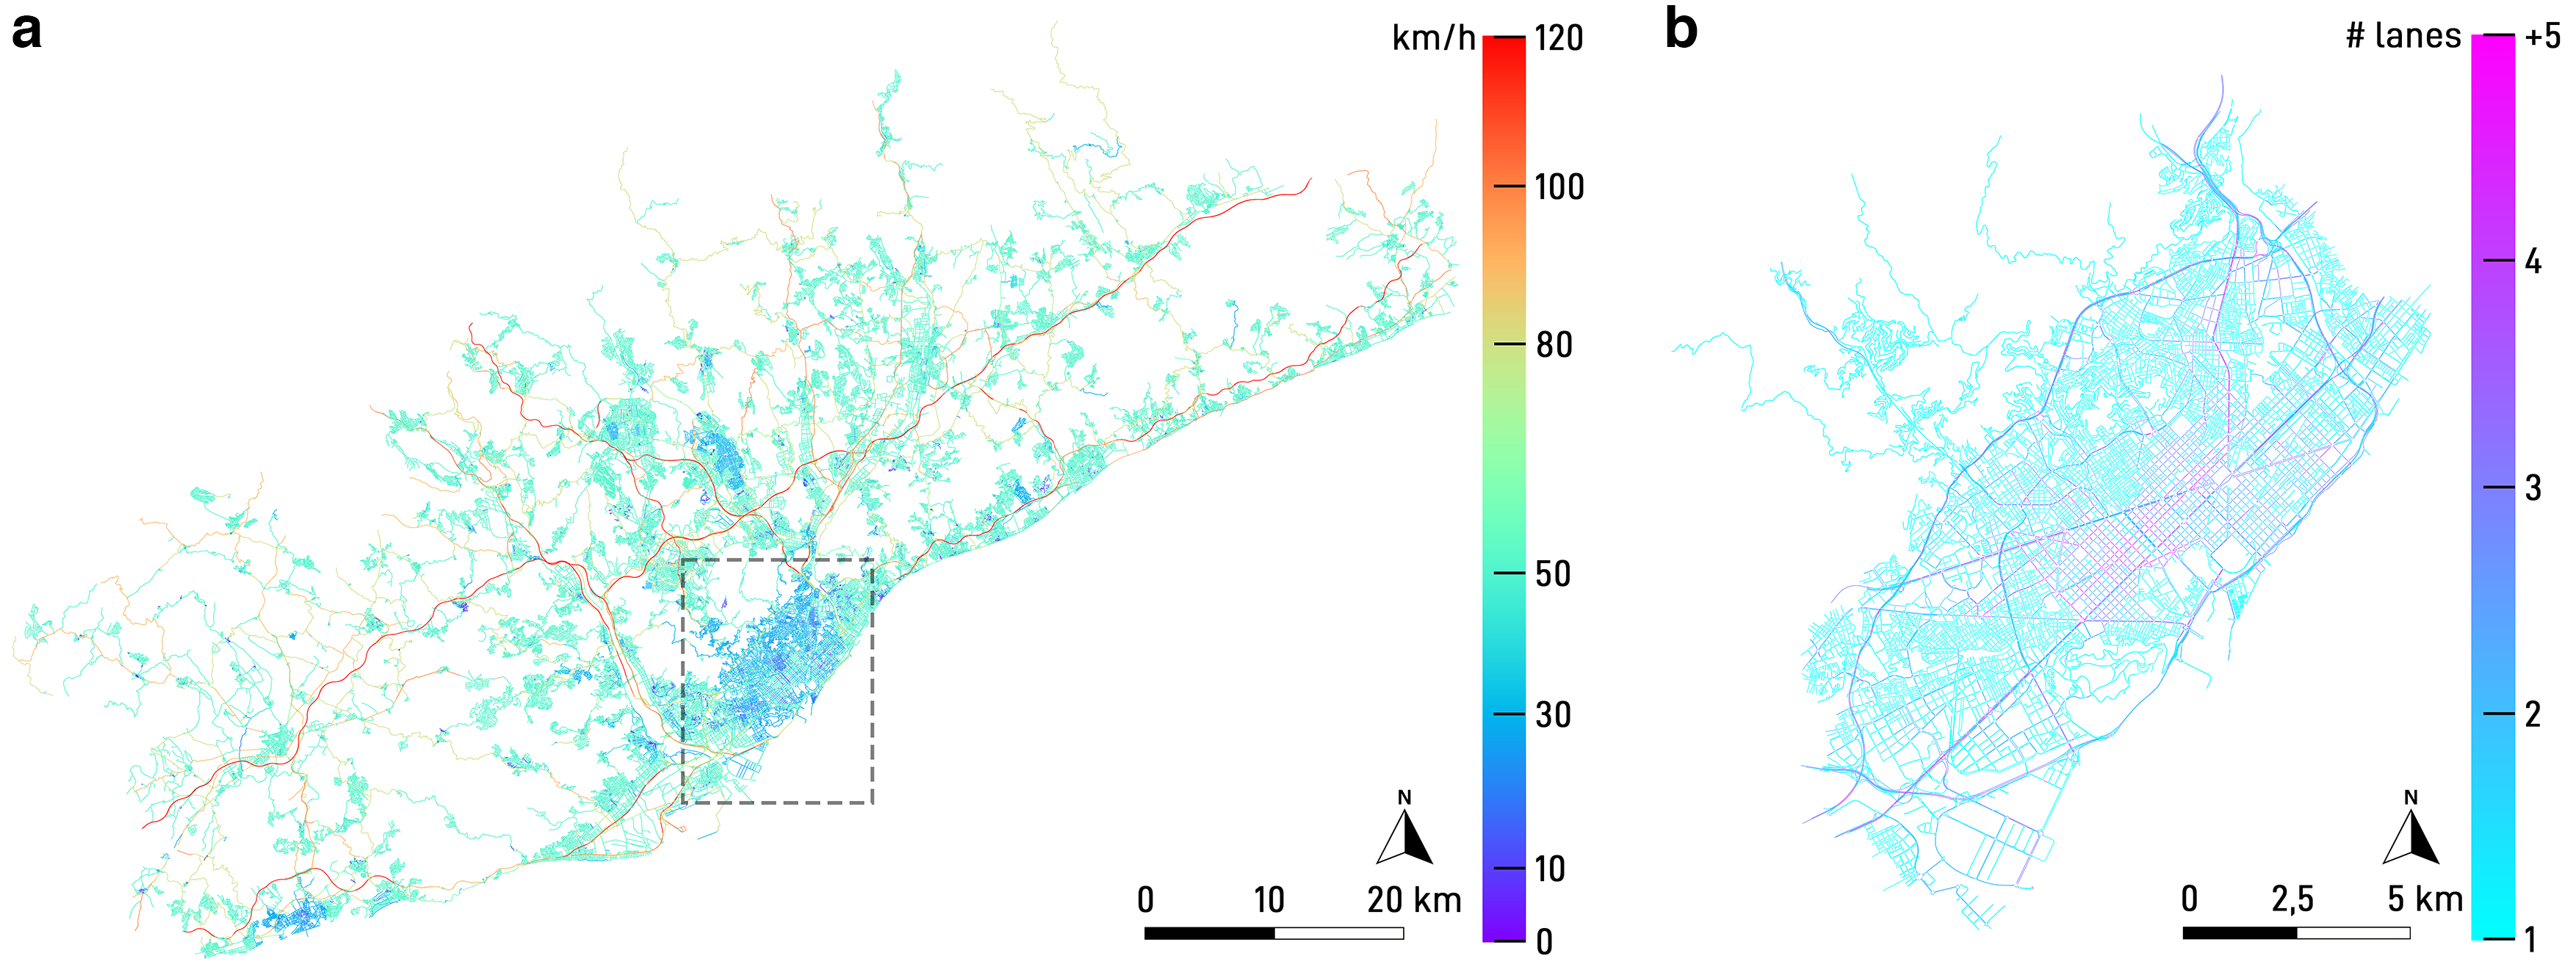
\includegraphics[width=1\textwidth]{fig_04.png}
    % \captionsetup{format=plain, justification=centering} % Center the caption
    \caption{Road network: (\textbf{a}) Network of the extended simulation area (RMB) showing speed limits in km/h; (\textbf{b}) Network of the core simulation area (Rondes) used for validating the detailed microsimulation, where different colours represent the number of lanes.}
   \label{fig:getting_real_04_road_net}
\end{figure}

% \usepackage{graphicx}
% \usepackage{booktabs}
% \usepackage{colortbl}


\begin{table}[hb!]
\centering
\caption{Features of the road networks.}
\label{tab:road_nets}
\arrayrulecolor{black}
\resizebox{\linewidth}{!}{%
\begin{tabular}{lcc} 
\toprule
\textbf{~}                        & \begin{tabular}[c]{@{}c@{}}\textbf{RMB }\\\textbf{ (Extended Area)}\end{tabular} & \begin{tabular}[c]{@{}c@{}}\textbf{\textit{Rondes} area }\\\textbf{ (Simulation Core)}\end{tabular}  \\ 
\hline
Area (km2)                        & 7726                                                                             & 182.55                                                                                               \\
Roads length (km)                 & 24,153.12                                                                        & 2,506.03                                                                                             \\
Lanes length (km)                 & 27,794.13                                                                        & 3,673.17                                                                                             \\
Number of links                   & 204,935                                                                          & 25,307                                                                                               \\
Number of
  intersections         & 98,752                                                                           & 13,993                                                                                               \\
Traffic lights                    & 3567                                                                             & 2035                                                                                                 \\
Traffic Assignment
  Zones (TAZs) & 577                                                                              & 296                                                                                                  \\
Virtual induction
  loops         & 10,496                                                                           & 10,496                                                                                               \\
\bottomrule
\end{tabular}
}
\arrayrulecolor{black}
\end{table}

\subsection{Demand Creation}

The approach followed in the demand generation aims to avoid underestimating real traffic flow, as it seems to happen in many microsimulations. In general, traffic within an area is expected to be caused by trips that have their origin or destination in that zone and also by through traffic originating and ending elsewhere. To deal with this situation, a basic spatial and temporal distribution of traffic is created for the extended simulation area (RMB) to identify the fraction of traffic that directly affects the core urban area (Rondes), which provides more realistic results than directly overlooking through traffic (see \autoref{fig:getting_real_07_performance_results} in \autoref{sec:GR_3_val} for comparing results without considering through traffic).

Two sources are used complementarily for the generation of traffic demand:

\begin{enumerate}
    \item Originally, traffic patterns are extracted from the origin/destination (O/D) matrices estimated from cell phone data \citep{Calvet2020,Caceres2007}. This method provides a direct estimation of flows between smaller areas (here areas refer to statistical zones used by the Catalan Institute of Statistics (IDESCAT). They are larger than census tracts, but smaller than districts or neighborhoods (see \autoref{fig:getting_real_02_geo_scope})) with finer granularity and larger sampling, overcoming limitations of estimations from self-reported surveys \citep{Caceres2020}. Given the focus on vehicular traffic, only the O/D matrix specific for daily private vehicle trips during a working day is considered, resulting from raw cell phone data processed based on the modal split from mobility surveys and public transit ridership data;
    \item Then, conventional mobility surveys \citep{InstitutdEstudisRegionalsiMetropolitansdeBarcelonaIERMB2020,AreadeBarcelona.AutoritatdelTransportMetropolita2020} are used complementarily to expand and correct the O/D matrix, in particular, to fill some gaps such as the actual hourly distribution of trips. It has been observed that the method to infer mobility patterns based on mobile phone location records tends to overestimate trips \citep{Calvet2020}.
\end{enumerate}
Thus, (1) the mobile phone data determine the detailed proportions of flows between the areas with a granularity unfeasible for survey data, while (2) the survey data determine the overall number of trips (which do not count partial trips separately, as cell phone data often do).

These O/D flows are spatially aggregated at the level of IDESCAT areas (see Figure 2). These areas considered as Transport or Traffic Analysis Zones (TAZs) are used for georeferencing the trips. SUMO provides the \emph{edgesInDistricts} script \citep{GermanAerospaceCenterDLRandOthers2021} to reference network edges to TAZs in such a way that origins and destinations of trips are linked to defined positions in the transportation network.

Initially, traffic demand is modelled for the entire extended area (RMB) using default parameters in SUMO. Later, all the O/D flows, which potentially may affect the core simulation area (Rondes), are kept, but peripheral traffic flows between the outer AMB and the outer RMB are ignored. This is also beneficial for computational performance.

As remarked, the main issues of these private vehicles’ O/D matrices from cell phone data are the overestimation of measured trips and the lack of disaggregated hourly distributions. Hence, inspired by data fusion approaches, which combine cell phone data with other sources \citep{Montero2019}, this model uses mobility surveys for complementing the O/D data. Particularly, these surveys provide hourly histograms of trips separated by RMB transport subareas and mode of transportation \citep{InstitutdEstudisRegionalsiMetropolitansdeBarcelonaIERMB2020}. This newly implemented method for O/D data correction and expansion is performed in two steps:

\begin{enumerate}
    \item TAZs are grouped by transport RMB subarea. Then, following the indications of the researchers in charge of the original analysis of the cell phone data, O/D flows are linearly scaled such that they match the number of trips for each of these subareas measured by the yearly mobility surveys \citep{InstitutdEstudisRegionalsiMetropolitansdeBarcelonaIERMB2020,AreadeBarcelona.AutoritatdelTransportMetropolita2020}, which are considered as accurate references in transport modelling and planning \citep{Montero2019}. Each subarea requires a different scaling, as the errors in the estimation of trips from cell phone data vary with trip length, population density, and the concentration of antennas \citep{Calvet2020,Caceres2020};
    \item The scale-corrected and hourly disaggregated O/D data obtained in the first step assume a symmetric number of trips between the different areas (i.e., outbound and in-bound trips are assumed to be equal in each hour of the day). This is unrealistic, of course (e.g., residential areas tend to emit more outbound trips in the morning towards working areas, while they tend to have more inbound trips in the afternoon and evening for returning commuters). To account for unbalanced flows between areas, the hourly histogram of trips is corrected by a factor based on skew-normal distributions for the peak hours of inbound and outbound trips in the morning and the afternoon/evening \citep{Melakessou2015}, which are computed using the Attraction and Emission Ratio (\emph{Ràtio d’atracció i emissió}, RAE) \citep{InstitutdEstudisRegionalsiMetropolitansdeBarcelonaIERMB2020}. Due to the lack of more disaggregated data, the trips staying within the same transport subarea are assumed to be symmetrically balanced throughout the day.
\end{enumerate}

As a result, 16 different O/D matrices are created for the pairwise relations between the four transport RMB subareas, accounting for inner, inbound, and outbound trips with their distinct hourly distributions. For instance, areas with lots of working places tend to have an inbound morning peak, and outbound afternoon or evening peaks.

In the next stage, all this time-series information is merged in SUMO, using \emph{od2trips} \citep{GermanAerospaceCenterDLRandothers2021b} with a timeline argument to convert raw O/D matrices into trips files referenced to the transportation network with the appropriate hourly distribution. The initial travel demand created by O/D matrices is defined by the time and edge of departure, and the destination edge in the network for each vehicle or trip. Unfortunately, this does not provide the whole path needed to identify which trips cross the core area. Therefore, \emph{duarouter} is used to route all trips with the Direct User Assignment (DUA) method \citep{GermanAerospaceCenterDLRandothers2021a}. Although this simple assignment approach only provides the optimum path when the network is empty (i.e., without considering changing traffic conditions and travel times throughout the day), it is used as a reference to create the initial distribution, which is adapted and optimized later.   

Once the DUA routing is performed for the extended area (RMB), SUMO’s \emph{cutRoutes} tool \citep{GermanAerospaceCenterDLRandothers2021} is used for cropping the resulting paths, which traverse the smaller but much denser network of the core area (Rondes). This is the scenario that is used for detailed analyses and simulations. Out of the 3,185,185 private vehicle trips initially computed for the whole extended RMB area, 2,063,177 trips turn out to cross some section of the core urban area of Barcelona (Rondes)  (see \autoref{tab:road_nets}). These are included in the final travel demand model.

\subsection{Calibration of Simulation Parameters}
\label{subsec:GR_2.4_cal_simu_params}

The numerous parameters involved in microscopic models and their long runtimes (around 30 h in this case) are troublesome for calibration \citep{Balakrishna2007}, making the use of the conventional simulation-based optimization \citep{Ciuffo2008} paradigm intractable \citep{alma990009089600205503}. This leads to compromises in realism. Initial tests identified that the aspects with the greatest impact on the simulation performance were the time step defining the temporal resolution, the car-following model chosen, and the procedure of rerouting:

\begin{itemize}
    \item The time step of the simulation needed to be reduced from 1 to 0.25 s to reproduce the continuous change of the traffic state sufficiently well \citep{Lieberman1996};
    \item Otherwise, the default parameters of Krauss’ car-following \citep{Krauss1997} and Erdmann’s lane-changing \citep{Erdmann2015} models in SUMO are used, adjusting the length of the vehicle to 4 m. This is closer to the average size of vehicles in Spain \citep{Mock2020} and also accounts for the exceptionally high proportion of motorbikes in Barcelona \citep{InstitutdEstudisRegionalsiMetropolitansdeBarcelonaIERMB2020,Marquet2016};
    \item Two parameters linked to routing are analysed: the probability for a vehicle to update its path during the simulation (\emph{device.rerouting.probability}) \citep{InTAS} and the factored priority of roads (\emph{weights.priority-factor}) as encoded in OSM data. To find their best values, different parameter combinations are explored by an algorithm that iteratively runs simulations for the \emph{device.rerouting.probability} with values between 0.6 and 1.0 in steps of 0.1 and for the \emph{weights.priority-factor} with values between 0 and 110 in steps of 10. The results are then compared based on the metrics used for the general evaluation of the model: number of teleports (``Teleporting'' is a mechanism that SUMO uses for avoiding agents,i.e., vehicles or pedestrians, to get indefinitely stuck in the simulation, by moving them to their following route edge, if they collided or are stopped for longer than a defined time period [86]\citep{GermanAerospaceCenterDLRandothers2021teleporting}. This ensures that minor specification errors do not mess up the entire simulation.), regression coefficient, R\textsuperscript{2}, RMSE, NRMSE, GEH for traffic counts, and DTW for the demand time series, see \autoref{sec:GR_3_val} for the explanation of the metrics. Consequently, the method obtains the minimum value for the errors ($RNMSE_{traffic\ counts} \approx 0.385$, $DTW_{hourly\ demand} \approx 3.5$) and maximum correlation coefficient for the linear regression ($coefficient \approx 0.91$, $R^2 \approx 0.81$) for $device.rerouting.\\probability = 1$ and $weights.priority-factor = 100$ (see \autoref{fig:getting_real_05_eval}).
\end{itemize}

\begin{figure}[htbp!]
    \centering
    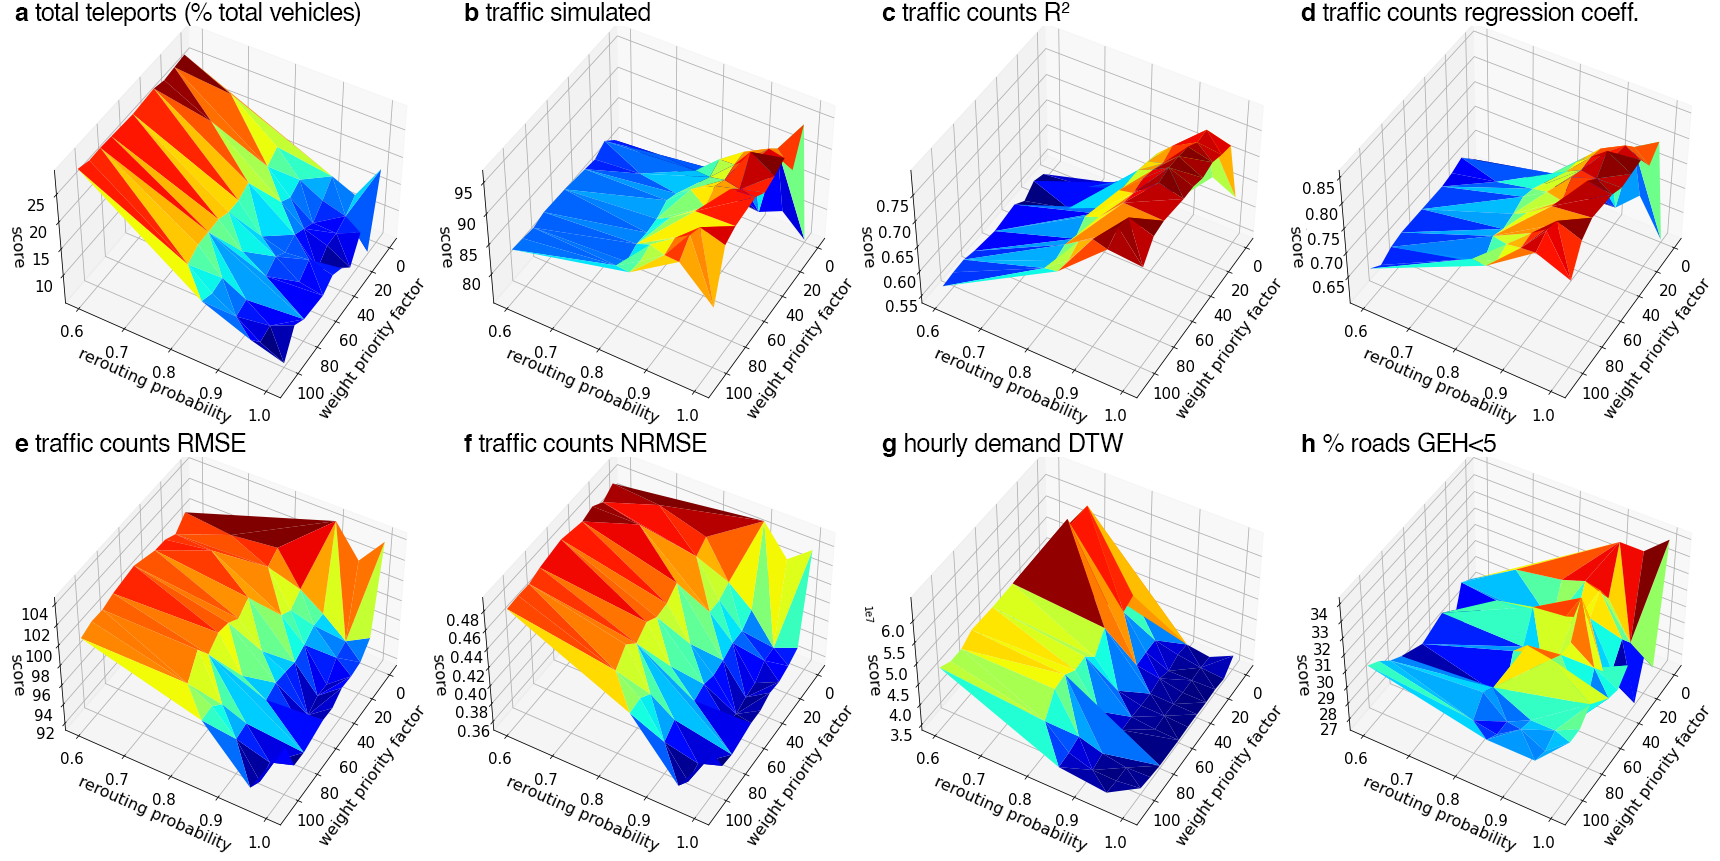
\includegraphics[width=1\textwidth]{fig05 copy.png}
    % \captionsetup{format=plain, justification=centering} % Center the caption
    \caption{Evaluation of the \emph{weights.priority-factor} and \emph{device.rerouting.probability}. Lower values for RMSE, NRMSE, and teleports are preferred, while higher values of the R\textsuperscript{2}, regression coefficient, and GEH indicate better performance: (\textbf{a}) Total teleports expressed in percentage of total vehicles loaded; (\textbf{b}) percentage of total demand effectively loaded into the simulation; (\textbf{c}) R\textsuperscript{2} coefficient between simulated and real traffic counts; (\textbf{d}) regression coefficient between simulated and real traffic counts; (\textbf{e}) RMSE between simulated and real traffic counts; (\textbf{f}) NRMSE between simulated and real traffic counts; (\textbf{g}) distance between theoretical temporal traffic demand curve and simulated based on DTW metric; (\textbf{h}) percentage of monitored links with a GEH statistic below 5.}
   \label{fig:getting_real_05_eval}
\end{figure}

\subsection{Demand Adaptation}
\label{subsec:GR_2.5_demand_adapt}

O/D pairs are the only source for the creation of traffic demand. It means that no ground truth regarding traffic counts, turning ratios, or other similar data is used to force the demand such that it matches reality. Instead, the results of the unconditioned adaptation are compared to the empirical “ground truth” to measure the quality of the model (see \autoref{sec:GR_3_val}).

The initial demand creation based on a Direct User Assignment (DUA) is simplistic because: (i) it does not account for the changing traffic conditions over the day (i.e., the fastest paths change depending on the congestion levels caused by other vehicles in the network), and otherwise (ii) it is found to be somewhat insufficient for large complex traffic scenarios. The process of demand adaptation tries to redistribute traffic realistically and efficiently in a time-dependent way. Frequently, in traffic simulations, this process is performed by Dynamic User Equilibrium (DUE) algorithms \citep{GermanAerospaceCenterDLRandothers2021e}, which expand Wardrop’s user equilibrium principle under the assumption that traffic tends to distribute spatially such that no single user can improve the travel time by changing the route \citep{Wardrop1952}. However, making route choices is mostly considered to be a probabilistic process, which rejects the assumption that drivers have a perfect and complete knowledge of the network to optimize their travel cost \citep{Daganzo1977}.

SUMO provides the \emph{duaIterate} tool to approximate the DUE \citep{GermanAerospaceCenterDLRandothers2021e} through an iterative optimization process that minimizes the overall travel time (or any other given cost function). In each run, a DUA is used to perform a whole simulation that allows computing the travel costs of edges, considering the changing congestion of the network loaded with traffic. Then, this is used to compute lower-cost paths, which is the basis of the DUA in the next iteration. By repeating this process many times, the algorithm tends to get closer to the equilibrium solution, which is imagined to be the best. Therefore, this paper extends for larger scenarios from previous approaches on heuristic dynamic assignment for achieving a stochastic user equilibrium \citep{Barcelo2006} by proposing two iterative optimization approaches using \emph{duaIterate}:

\begin{itemize}
    \item In-Simulation Adaptive Rerouting (iSAR) uses the capabilities of SUMO to allow vehicles to update automatically their paths during the simulation to find a faster route based on existing traffic conditions. This approach does not seek directly for a DUE but tries to adapt traffic efficiently, using a very fast adaptive strategy. Additionally, integrating this method into the \emph{duaIterate} routine allows checking the stability of the results. It might be possible to improve the performance of the traffic assignment even further by identifying underlying structures in the evolution of the travel costs of the network, although it is expected that reactive rerouting during simulation could address many of these effects;
    \item Iterative Incremental Dynamic User Equilibrium (IIDUE) depends exclusively on \emph{duaIterate} to run the simulation and the DUA repeatedly and to adapt the traffic distribution based on newly found optimal travel costs in each iteration. However, due to the high level of congestion in this scenario, it is not possible to simulate the whole traffic demand from the beginning. The oversaturation and gridlock caused by the initial, trivial DUA do not generate informative travel cost values for edges suitable for the optimization process. To overcome this limitation, this approach implements an incremental assignment strategy. Starting with 2\% of the overall traffic demand, an additional 2\% of trips are added in each iteration to allow the algorithm to gradually account for changing travel costs, before reaching unrecoverable and uninformative congestion. On the other hand, this process is time-consuming, that is, slow and computationally expensive.
\end{itemize}

To compute the probability of choosing a new route based on cost optimization in every single iteration, \emph{duaIterate} offers two different methods, which are compared: \textbf{Gawron} and \textbf{Logit}. Both approaches take as inputs a weight or cost function $w$ for the edges, a set of routes $R$, and for each of these routes $r$, an old cost $c_r$, an old probability $p_r$, and a new cost $c_{r}’$ and probability $p_{r}’$ \citep{GermanAerospaceCenterDLRandothers2021e}. The two methods differ on how they update these new values in every simulation iteration:

\textbf{Logit} is simpler. It uses an explicit analytical formula to compute the new probability directly by only considering the sum of the costs of all edges $e$, which are part of the route $r$ in the last iteration:
\begin{align}
    c'_r = \sum_{e \in r} w(e) \label{eq:logit}
\end{align}

Then, the probabilities are updated, using an exponential distribution containing a parameter $\theta$, and normalized by the sum over all routes s in the set $R$:
\begin{align}
    p'_r = \frac{\exp(\theta c'_r)}{\sum_{s \in R} \exp(\theta c'_s)} \label{eq:logit_update_prob}
\end{align}

However, in this paper, a generalization of the logit model named \emph{c}-Logit \citep{Cascetta1996} is used, which is defined by
\begin{align}
    p'_r = \frac{\exp(\theta (c'_r + \text{cf}'_r))}{\sum_{s \in R} \exp(\theta (c'_s + \text{cf}'_s))} \label{eq:c-logit}
\end{align}

This gives more realistic route choice probabilities, which consider a commonality term $cf'_r$ that accounts for the overlap of alternative paths (this is particularly relevant given the regular grid of Barcelona that may lead to many similar overlapping alternatives), specified by
\begin{align}
   cf'_r = \beta \ln \sum_{s \in R} \left( \frac{L_{rs}}{\sqrt{L_r} \sqrt{L_s}} \right)^\gamma \label{eq:c-logit_overlap_paths}
\end{align}

Herein, $L_{rs}$ is the length of edges shared by routes $r$ and $s$, respectively, with total lengths $L_r$ and $L_s$. $\beta$ and $\gamma$ are parameters (when $\beta=0$, \emph{c}-logit becomes the simpler logit model). The models in this paper use a value of $\beta=0.15$ and $\gamma=1$ (the default in SUMO).

\textbf{Gawron} computes the probability for choosing a new route from a set of alternatives, based on the travel time (or any other cost function) of the route chosen in the previous iteration. It further considers the sum of travel times of these alternatives and the previous probability of choosing a route \citep{Gawron1999}. After each simulation iteration, travel times are updated according to

\begin{align}
   \tau'_d(x) = \begin{cases} \tau_s(x) & \text{if route } x \text{ was simulated} \\ \beta \tau_r(x) + (1 - \beta)\tau_d(x) & \text{otherwise} \end{cases} \label{eq:GR_gawron}
\end{align}

Herein, for a given route x, $\tau_s(x)$ is the simulated travel time, $\tau_r(x)$ is the estimated travel time from the simulation for other routes not used in the iteration, and $\beta$ is a remembering factor for scaling the impact of costs of past unused routes. Then, the probabilities are updated according to

\begin{align}
   p'_d(r) = \frac{p_d(r) \left(p_d(r) + p_d(s)\right) \exp\left(\frac{\alpha \delta_{rs}}{1 - \delta_{rs}^2}\right)}{p_d(r) \exp\left(\frac{\alpha \delta_{rs}}{1 - \delta_{rs}^2}\right) + p_d(s)} \label{eq:GR_gawron_prob_update1}
\end{align}

and

\begin{align}
   p'_d(s) = p_d(r) + p_d(s) - p'_d(s) \label{eq:GR_gawron_prob_update2}
\end{align}

where $p_d (x)$ and $p'_d (x)$ are the prior and new probabilities to use route $x$, $r$ is the route used in the previous simulation iteration, $s$ another route in the set of alternatives $R$, and $\delta_{rs}$ is the relative cost difference between routes $r$ and $s$ defined by

\begin{align}
   \delta_{rs} = \frac{\tau_d(s) - \tau_d(r)}{\tau_d(s) + \tau_d(r)} \in [-1, 1] \label{eq:GR_gawron_delta_rs}
\end{align}
$\tau_d (s)$ represents the travel time for driver d to complete route $x$. In this scenario, SUMO’s default values are used for Gawron’s parameters, namely $\alpha=0.5$ and $\beta=0.9$.

\section{Results Validation}
\label{sec:GR_3_val}

It is not possible to formally prove the convergence of the proposed heuristic dynamic traffic assignment approaches as there is no analytical solution for the loading process in microsimulations \citep{Barcelo2006,Batty2013}. Therefore, an extensive multi-variable evaluation over the 24 h of a generic weekday allows test empirically many of the different aspects of the goodness-of-fit between simulation and reality at different levels and scales. Based on the re-viewed literature regarding traffic simulation evaluation, the chosen performance metrics can be classified according to their different levels of spatial and temporal aggregation (\autoref{fig:getting_real_06_class_eval_vars}). However, as already pointed out in previous research, the possibilities of evaluation are limited by the availability of real data serving as ground truth and different from the ones used for demand generation.

\begin{figure}[htbp!]
    \centering
    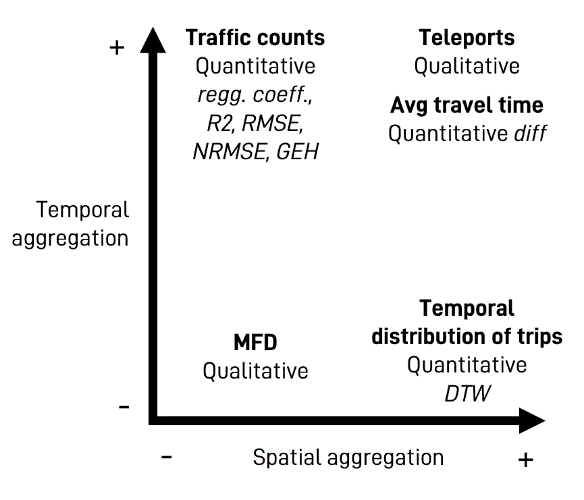
\includegraphics[width=0.5\textwidth]{fig_06.png}
    % \captionsetup{format=plain, justification=centering} % Center the caption
    \caption{Classification of evaluation variables and metrics based on their spatio-temporal aggregation (based on the framework proposed in \citep[Figure 1]{Kang2019})}
   \label{fig:getting_real_06_class_eval_vars}
\end{figure}

\subsection{Large-Scale Aggregated Metrics: Teleports and Average Travel Time}

Let us start by looking at the most aggregated metrics: "Teleporting" has no correspondence to a real measurement, but constitutes a first sanity check of the simulation, as a large proportion of vehicles teleporting means a poor model performance. In general, iSAR shows a reasonable number of teleports (around 5\%), with lower variability than the teleports resulting from the IIDUE method (see \autoref{fig:getting_real_07_performance_results}a,b).
On the highest level of aggregation, the average travel times between simulation and reality are compared. Mobility surveys provide information regarding the average duration of trips for different subareas of the RMB and separated by mode of transport. The inner Metropolitan Area, which roughly corresponds to the core area of the simulation (Rondes), has an average travel time for private vehicles of 23.5 min (or 1410 s) \citep{InstitutdEstudisRegionalsiMetropolitansdeBarcelonaIERMB2020}. This value is very similar to the results of the simulations based on the iSAR approach (around 1400 s); while the average travel times resulting from the IIDUE method deviate considerably (see \autoref{fig:getting_real_07_performance_results}c).

\begin{figure}[htbp!]
    \centering
    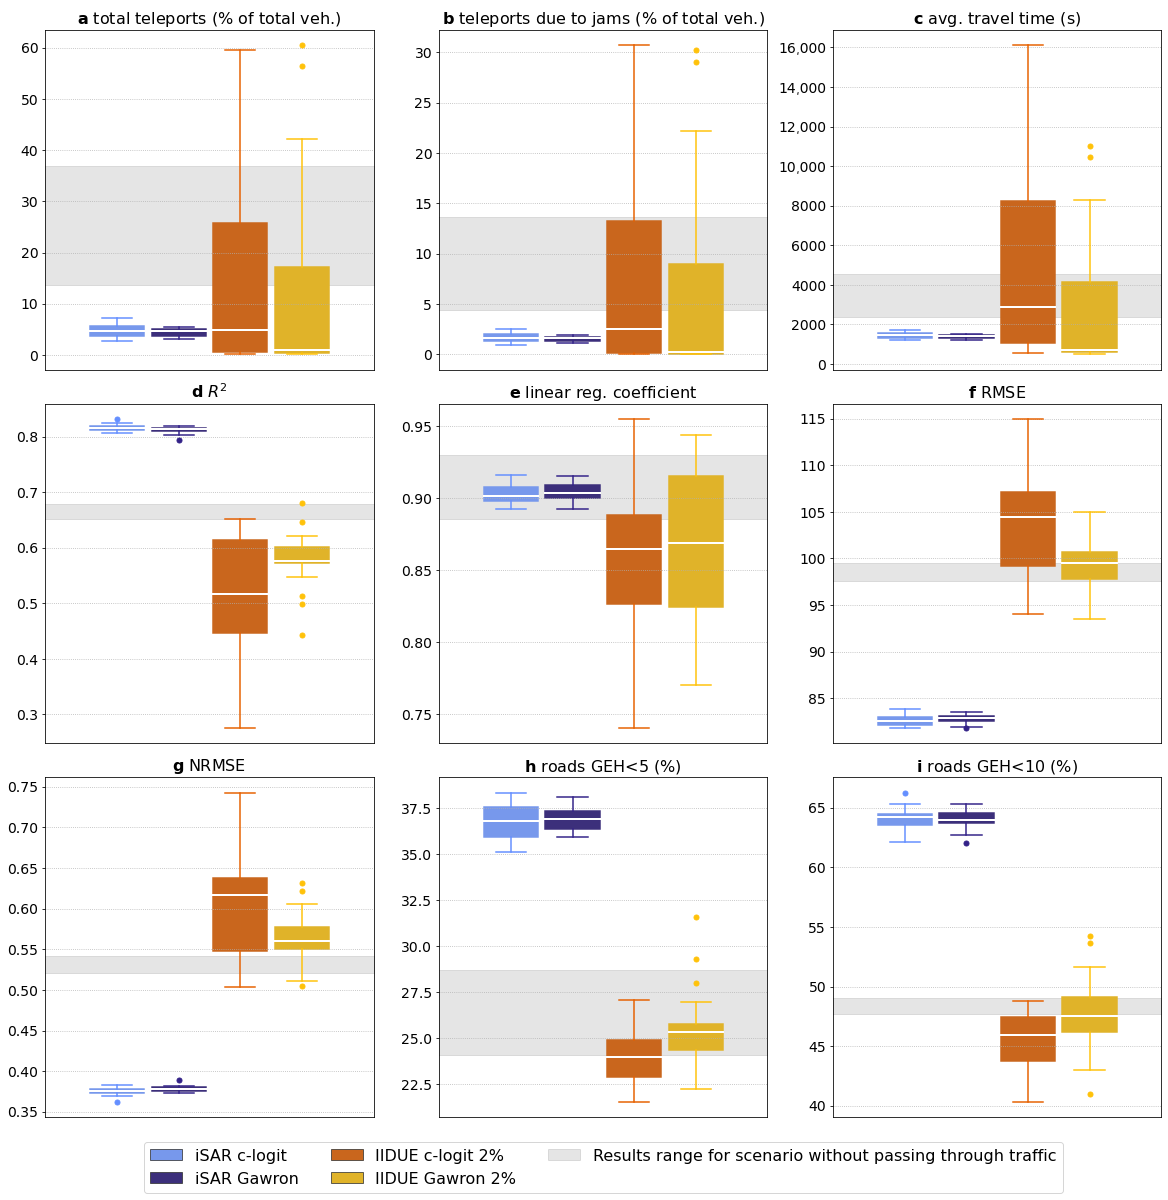
\includegraphics[width=1\textwidth]{fig_07.png}
    % \captionsetup{format=plain, justification=centering} % Center the caption
    \caption{Performance of the analysed models (for the core simulation area, Rondes). iSAR outperforms IIDUE results: it shows more stable results, closer to measured average travel time, better goodness of fit, and lower error measures. Shaded ranges show the model’s underperformance when not considering passing through traffic (i.e., crossing Rondes core area): (\textbf{a}) Total teleports expressed in percentage of total vehicles loaded; (\textbf{b}) Teleports caused by jams, expressed in percentage of total vehicles loaded; (\textbf{c}) Average travel times for all vehicles in seconds; (\textbf{d}) R\textsuperscript{2} coefficient between simulated and real traffic counts; (\textbf{e}) regression coefficient between simulated and real traffic counts; (\textbf{f}) RMSE between simulated and real traffic counts; (\textbf{g}) NRMSE between simulated and real traffic counts; (\textbf{h}) percentage of monitored links with a GEH statistic below 5; (\textbf{i}) percentage of monitored links with a GEH statistic below 10.}
   \label{fig:getting_real_07_performance_results}
\end{figure}

\subsection{Temporally Disaggregated Metrics: Hourly Distribution of Trips}

With a higher level of temporal disaggregation, the hourly distribution of trips throughout the day is as well compared (\autoref{fig:getting_real_08_tempo}). For the ground truth, mobility surveys provide 24-h temporal histograms of when trips begin, differentiated by RMB subareas and mode of transportation \citep[page 59]{InstitutdEstudisRegionalsiMetropolitansdeBarcelonaIERMB2020}.

\begin{figure}[htbp!]
    \centering
    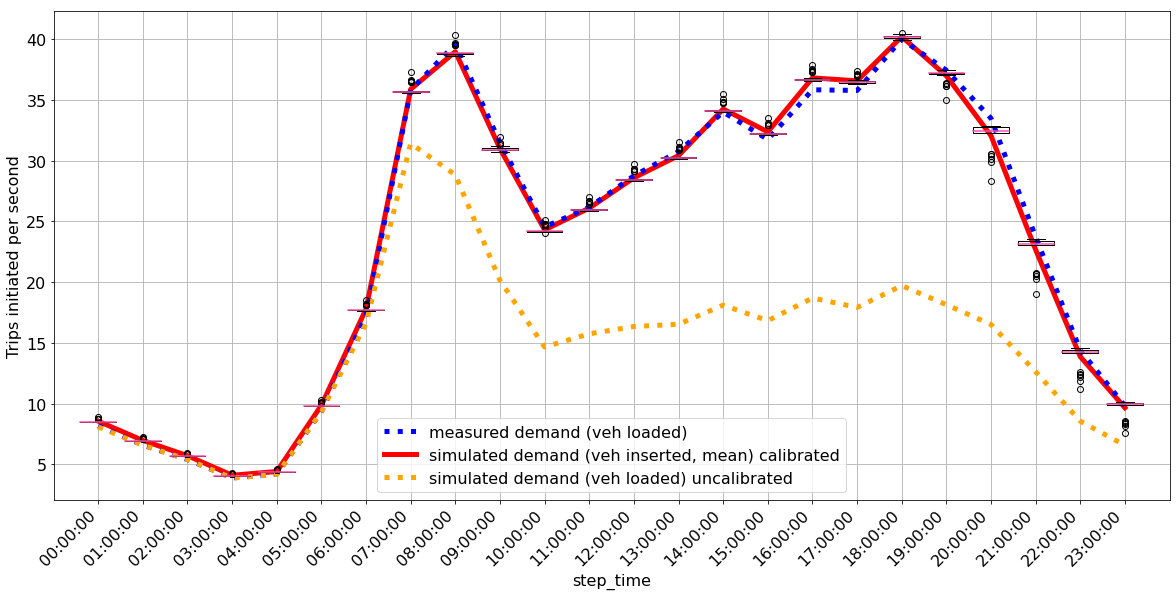
\includegraphics[width=1\textwidth]{fig_08.png}
    % \captionsetup{format=plain, justification=centering} % Center the caption
    \caption{Temporal distribution of trips showing the measured demand in surveys ("ground truth", dotted blue curve) as compared to the simulated demand (red solid line) after parameter calibration (\autoref{subsec:GR_2.4_cal_simu_params}) and adaptation (\autoref{subsec:GR_2.5_demand_adapt}), with boxplots showing variations across iterations. The dotted orange line shows the results of the simulation without calibration.}
   \label{fig:getting_real_08_tempo}
\end{figure}

When scenarios are close to congestion, programmed trips may not find enough space in the transport network to be inserted, such that they are delayed or eventually even skipped. This can potentially lead to different demand curves or an overall lower processed demand (see the uncalibrated simulated demand in \autoref{fig:getting_real_07_performance_results}). Dynamic Time Warping (DTW) \citep{Bellman1958} with the \emph{FastDTW} implementation \citep{Salvador2007} is used to compare real and simulated temporal distributions. This technique allows finding the similarities between two time series by non-linearly distorting the time axis, which becomes very useful when divergences are caused by different speeds, frequencies, and phasing as they may particularly occur in the case of network (over)saturation. Overall, there is a good match between simulation and ground truth, with low variability, showing clearly the observed morning and early evening peaks. The DTW distance value stays very stable across the successive iterations with a value around 19,000. However, in general, we can consistently observe a slightly lower simulated demand, particularly in peak hours, most likely due to high levels of congestion that prevents some vehicles to be inserted in the network at the expected time, which are eventually skipped.

\subsection{Spatially Disaggregated Metrics: Traffic Counts}

Traffic counts provide a spatially disaggregated evaluation. The city of Barcelona has 488 permanent traffic counting stations (see \autoref{fig:getting_real_09_traffic_counts}a). However, only Monthly Average Daily Traffic (MADT) counts are publicly available [96]\citep{AjuntamentdeBarcelona2019gauging}. Other metrics such as temporal distributions of trips for each detector [85] and average speeds \citep{Rodriguez-Rey2021,Yu2017}, which have been used effectively for more detailed assessments in other scenarios, were not available.

\begin{figure}[htbp!]
    \centering
    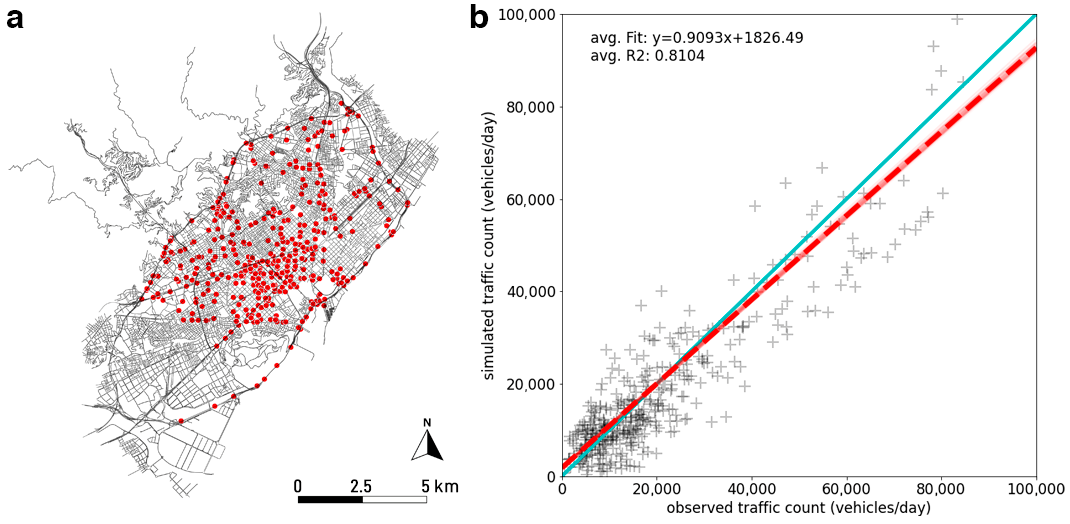
\includegraphics[width=1\textwidth]{fig_09.png}
    % \captionsetup{format=plain, justification=centering} % Center the caption
    \caption{Traffic counts: (\textbf{a}) Location of the 488 AADT detectors managed by the city of Barcelona, which are used to assess the quality of the model calibration; (\textbf{b}) Regression plot comparing real and simulated traffic counts (averaged over all the iSAR simulations using the c-Logit and Gawron methods). R\textsuperscript{2} > 0.8 is considered a good fit.}
   \label{fig:getting_real_09_traffic_counts}
\end{figure}

The large variability of observed monthly averages throughout the year in some of the control points (see \autoref{fig:getting_real_10_traffic_counts_locations}) creates a wide range of possible correct matchings with the ground truth, particularly as the timestamps of the cell phone tracks used for generating the traffic demand are unknown. To address this limitation, the monthly averages are aggregated to annual averages (AADT). Values within 1 standard deviation of this average are considered to be a good fit.

Linear regression is used to evaluate the general goodness-of-fit between simulated and real measurements of traffic counts (see \autoref{fig:getting_real_09_traffic_counts}b). iSAR simulations results show a slope of 0.91 and an $\text{R}^2$ value of 0.81 (see \autoref{fig:getting_real_07_performance_results}d,e), which can be considered a good match \citep{MinisteriodeFomento2014}. Again, the results from the IIDUE method reach worse values for both metrics.

\begin{figure}[htbp!]
    \centering
    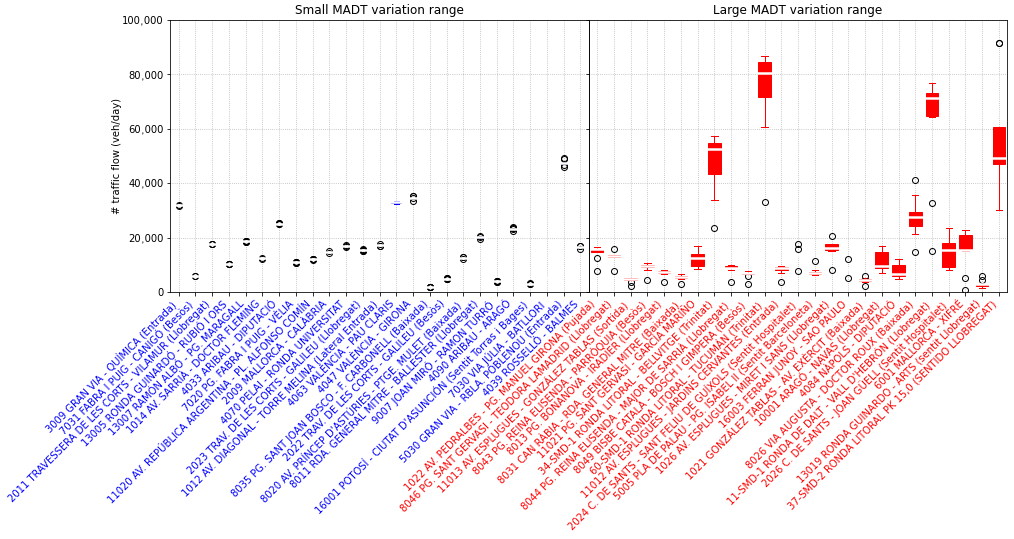
\includegraphics[width=1\textwidth]{fig_10.png}
    % \captionsetup{format=plain, justification=centering} % Center the caption
    \caption{Measured traffic counts at selected locations showing Monthly Average Daily Traffic counts (MADT) ranges with the 25 control points where the normalized variability ($normalized\ range_{MADT}=(abs(max_{MADT}-min_{MADT}))⁄\overline{MADT}$) is lowest (left, in blue) and highest (right, in red).}
   \label{fig:getting_real_10_traffic_counts_locations}
\end{figure}

A second set of metrics regarding traffic counts offers a more detailed evaluation. Among the many available model performance statistics reflecting different aspects of the discrepancies between predictions and ground truth, three of the most common ones across recent literature are selected \citep{Balakrishna2007,Yu2017} (see \autoref{tab:large_scale_traffic_simulation_examples}): the general Root Mean Square Error (RMSE), a Normalised Root Mean Square Error (NRMSE), and the Geoffrey E. Harvers statistic (GEH).
The RMSE and NRMSE are specified as

\begin{align}
   \text{RMSE} = \sqrt{\frac{\sum_{i=0}^n (S_i - O_i)^2}{n}} \label{eq:RMSE}
\end{align}

\begin{align}
   \text{NRMSE} = \frac{\sqrt{\frac{\sum_{i=0}^{n} (S_i - O_i)^2}{n-1}}}{\frac{\sum_{i=0}^{n} O_i}{n}} \label{eq:NRMSE}
\end{align}

where n is the number of observation points, and $O_i$ and $S_i$ are the real observed and simulated values of traffic counts at location i, respectively. RMSE is sensitive to scale, so it allows the comparison of both assignment methods for the two route choice methods as they use the same traffic demand. The iSAR method shows lower and more stable RMSE values, which is better than the IIDUE approach, with no relevant differences between the \emph{c}-Logit and Gawron methods (see \autoref{fig:getting_real_07_performance_results}f).

RMSE normalization allows for a more general and scale-independent (i.e., da-ta-independent) comparison between models. The mean of the real observations is chosen as the normalization criterion for the NRMSE approach. It reports values in the range [0,1], so multiplying it by 100 generates a percentage-like score (known as well as NRMSE or \%RMSE). According to the established literature \citep{MinisteriodeFomento2014,He2018,Li2015}, any value below 0.3 (or 30\%) can be considered good. In the case of the presented models, the iSAR simulations outperform again the results of the IIDUE method (see \autoref{fig:getting_real_07_performance_results}g) but even in the best scenario, the values are above 0.3, so the model performance is limited.

The previously considered metrics (i.e., regression’s coefficient, $\text{R}^2$, RMSE, and NRMSE values), which are commonly used for the performance evaluation of (simulation and prediction) models in many fields, does not work particularly well for the case of complex transportation networks with highly variable network elements \citep{Balakrishna2007}. To overcome this problem, the Geoffrey E. Harvers statistic (GEH), which is a modified chi-squared metric, is frequently used in traffic studies. It leverages relative and absolute differences to compute percentage errors regarding the mean value of observed and simulated traffic counts. The GEH statistic is defined by
\begin{align}
   \text{GEH} = \sqrt{\frac{(S - O)^2}{\frac{S + O}{2}}} \label{eq:GEH}
\end{align}

where $S$ is the simulated traffic count, and $O$ is the real observed traffic count \citep{DepartmentforTransportUKGovernment2020,Dowling2004}. GEH values below 5 are considered a good fit, values between 5 and 10 are ok, but need further checks, and GEH values over 10 are a bad match. Ideally, 85\% or more of the observed links should have a GEH value below 5. None of the resulting models reaches this score, which is consistent with the analysed previous large-scale urban microsimulations. However, iSAR performs better, having 38\% of the analysed links with a GEH smaller than 5, where the differences between the Gawron and $c$-Logit approaches are negligible (see \autoref{fig:getting_real_07_performance_results}h,i).

\subsection{Macroscopic Metrics: MFD}

Finally, macroscopic fundamental diagrams (MFD) \citep{Geroliminis2008} provide an additional perspective for the evaluation of the generated models. However, in contrast to the previous quantitative tests, this check is qualitative. The lack of empirical data and the discrepancies in estimations for real scenarios \citep{Ambuhl2017} are still a challenge for their use. Nonetheless, one can make an additional assessment with them. The obtained MFD (\autoref{fig:getting_real_11_MFD}) features the characteristic inverse-$\lambda$ form \citep{Treiber2013}, with capacity values compatible with measured capabilities for different roadways typologies \citep{Hall1996}.

\begin{figure}[htbp!]
    \centering
    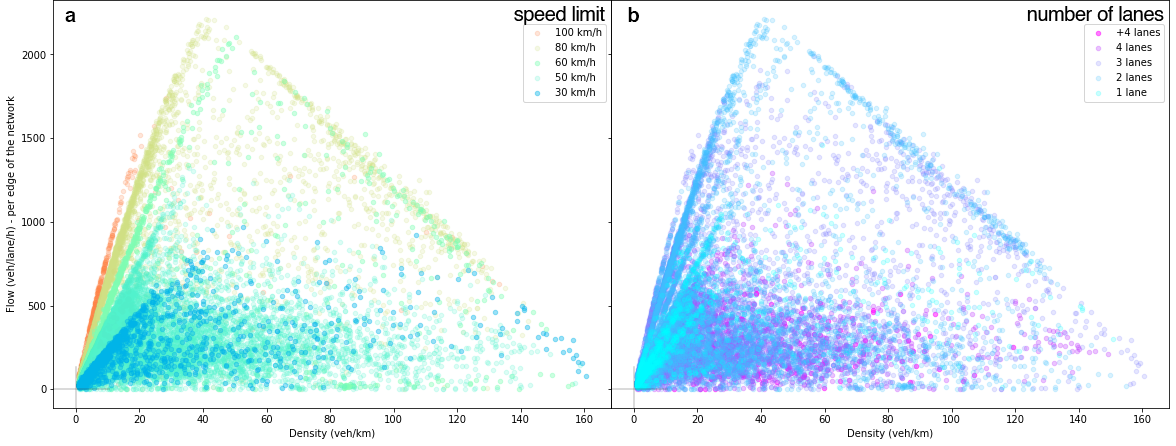
\includegraphics[width=1\textwidth]{fig_11.png}
    % \captionsetup{format=plain, justification=centering} % Center the caption
    \caption{Obtained Macroscopic Fundamental Diagrams values with the microsimulation: (\textbf{a}) coloured based on the speed limit of the road section; (\textbf{b}) coloured based on the number of lanes of the road section.}
   \label{fig:getting_real_11_MFD}
\end{figure}

\section{Discussion and Outlook}
\label{sec:GR_4_dis}

In this paper, a new large-scale traffic microsimulation for the urban area of Barcelona using the software SUMO is presented. It combines novel and more precise origin-destination matrices estimated from anonymized mobile phone records with traditional mobility surveys on a network extracted from OpenStreetMap. The resulting model shows a good level of correspondence with reality (see \autoref{fig:getting_real_12_result_summary}), outperforming previous examples, after being widely validated by metrics on different scales. It expands the state-of-the-art of traffic simulation by pushing microscopic approaches into large-scale scenarios supported by real data to obtain an operationally realistic and efficient model that can assess citywide impacts at fine-grained detail of policy decisions. Simultaneously, it allows identifying the limitations of these modelling approaches when considered within the concept of “urban digital twins”.

\begin{figure}[htbp!]
    \centering
    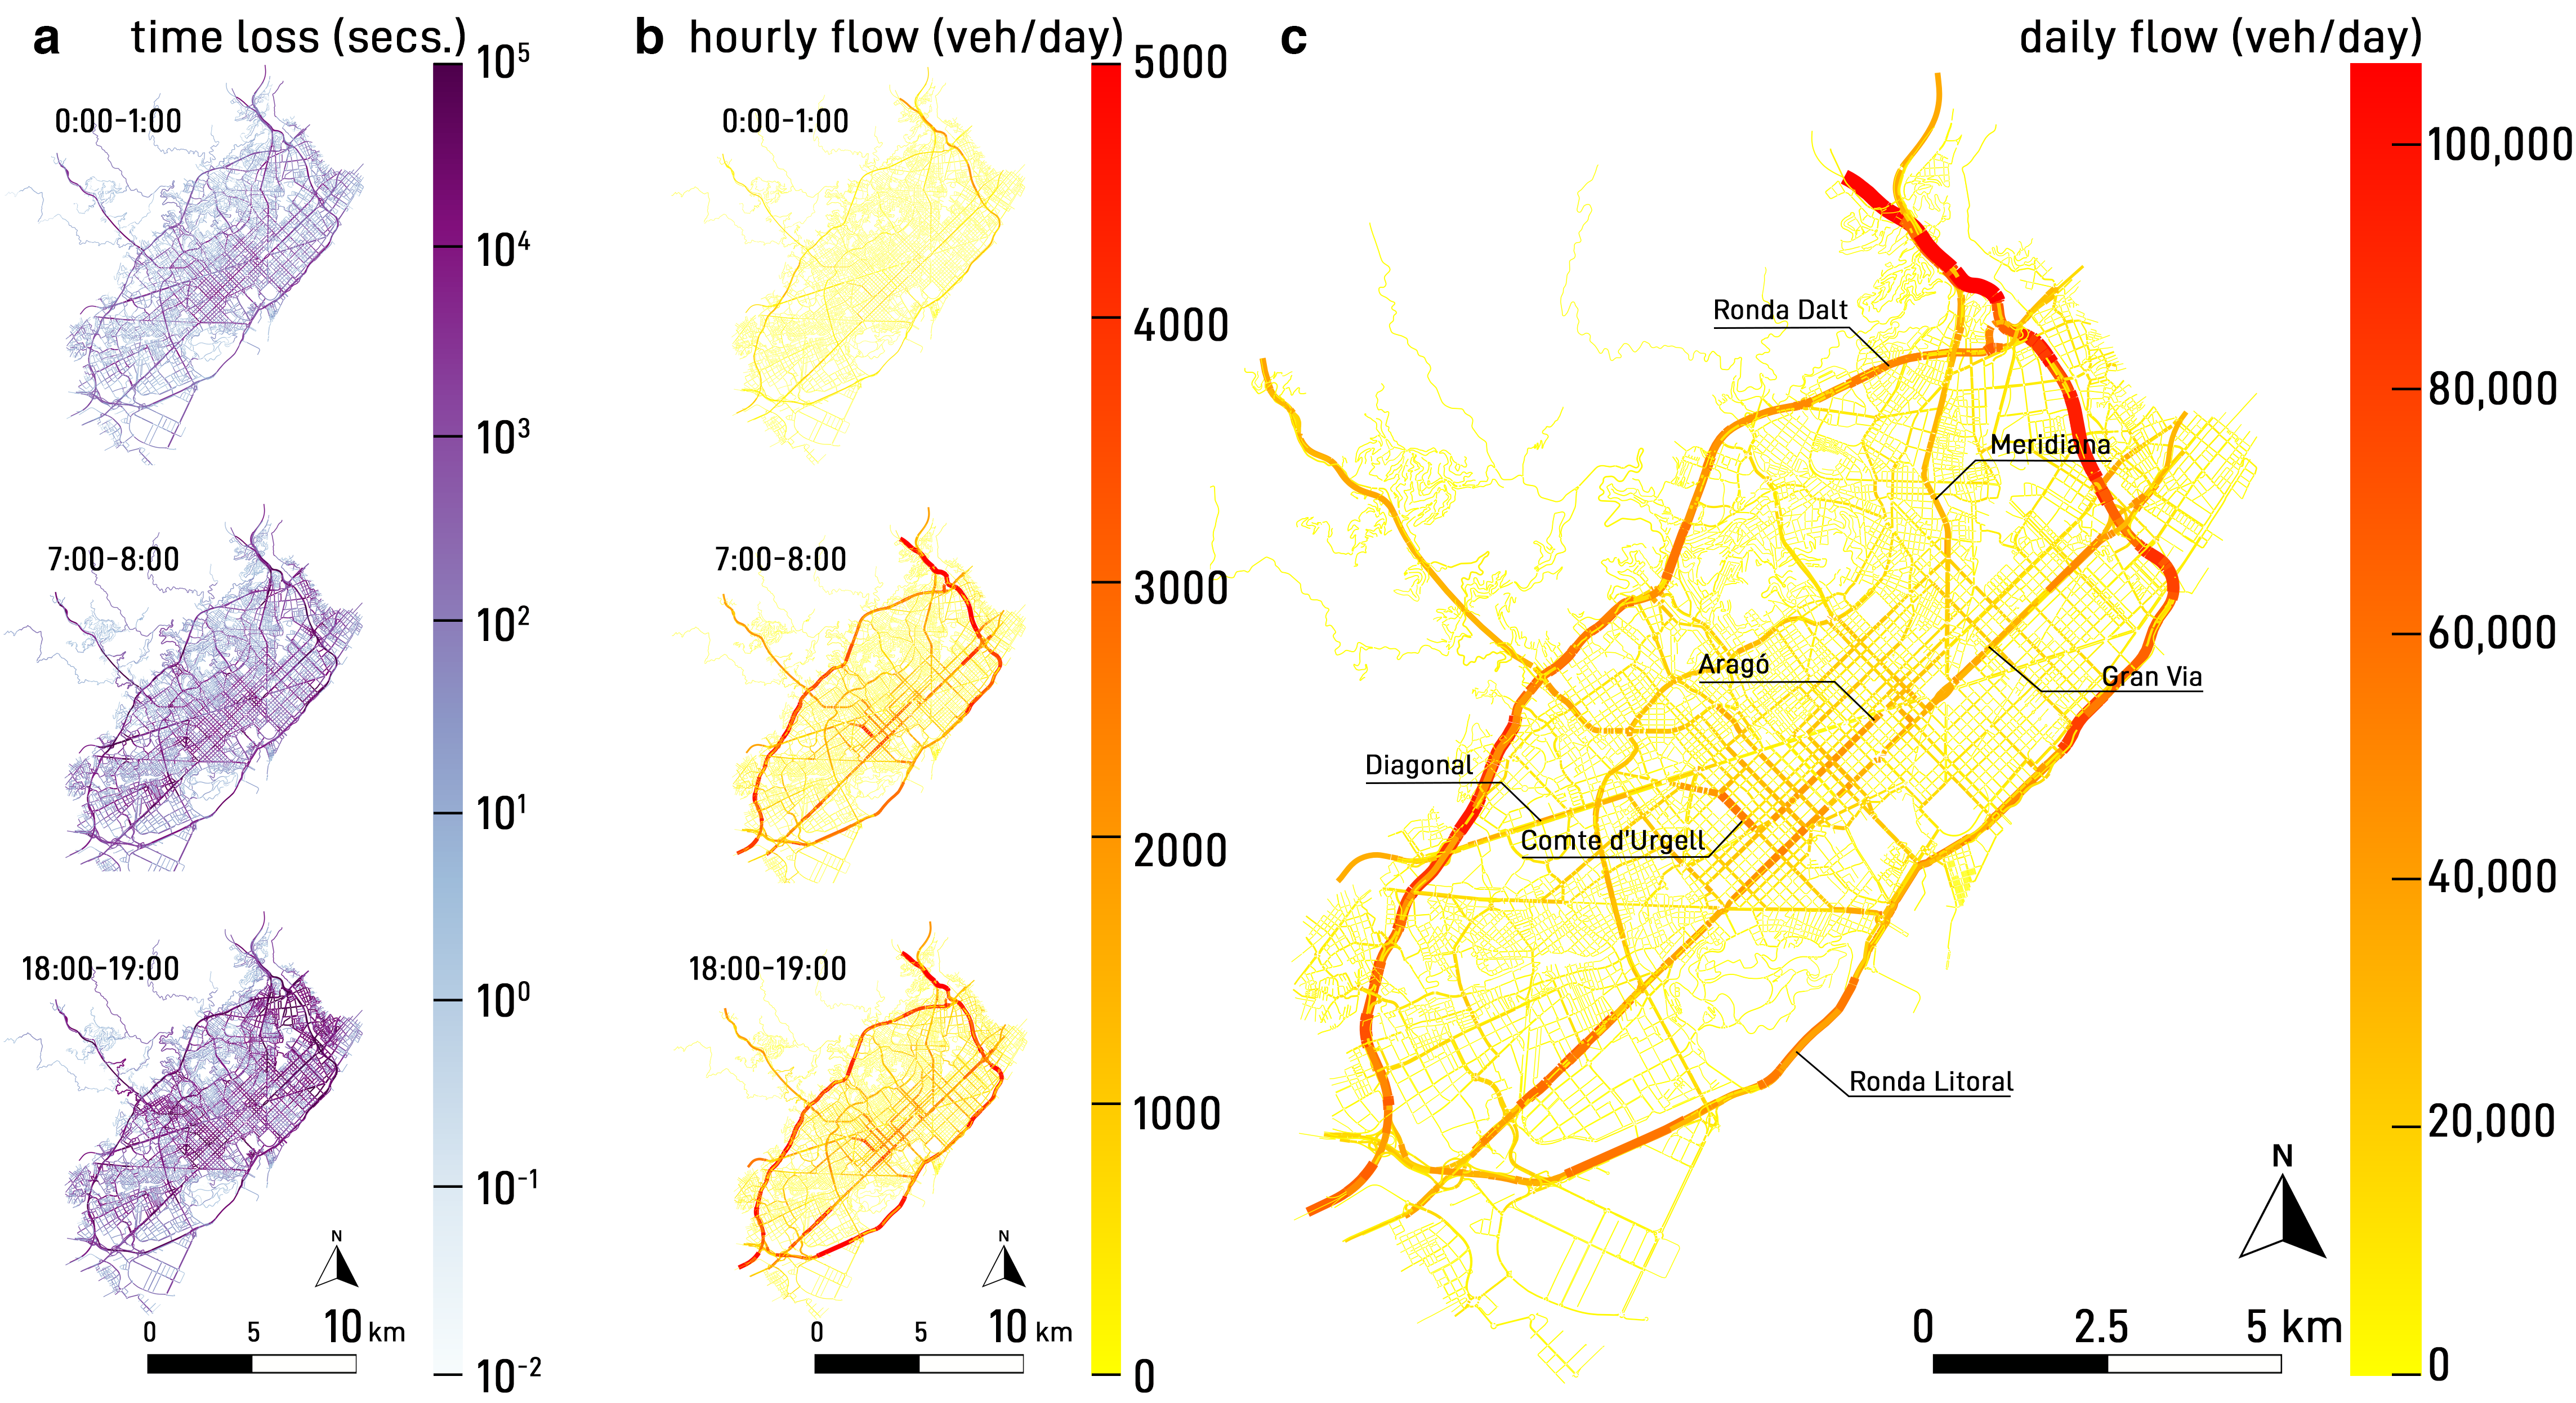
\includegraphics[width=1\textwidth]{fig_12.png}
    % \captionsetup{format=plain, justification=centering} % Center the caption
    \caption{Simulation results: (\textbf{a}) Congestion level measured by aggregated loss of time in seconds in 3 relevant intervals (off-peak plus morning and evening peak hour); (\textbf{b}) Congestion level measured by aggregated traffic counts in 3 relevant intervals (off-peak plus morning and evening peak hour); (\textbf{c}) 24 h traffic counts.}
   \label{fig:getting_real_12_result_summary}
\end{figure}

The calibration of the model identified the simulation time step, the probability for the vehicles to reroute during the simulation, and the influence of the edge priority as the most relevant factors without having to perform an exhaustive exploration of the huge parameter space, which often makes the calibration and use of these models impractical.

Two approaches (in-Simulation Adaptive Rerouting, iSAR, and Iterative Incremental Dynamic User Equilibrium, IIDUE), under two route choice algorithms (Gawron and \emph{c}-Logit), were compared to tackle the challenge of distributing a high traffic demand in a dense and complex large urban network. The lack of analytical form in this microsimulation approach requires an extensive multi-variable empirical evaluation to check their performance comparing real and simulation data on different spatial and temporal scales. These different quantitative metrics included the average trip duration, the similarity of temporal distributions of trips using DTW, and the comparison of simulated and real traffic counts based on the linear regression coefficient, R\textsuperscript{2}, RMSE, NRMSE, and GEH statistics. Additionally, two qualitative tests based on simulation "teleports" and MFDs are included.

iSAR outperforms IIDUE in all the metrics without relevant differences between the \emph{c}-Logit and Gawron’s approaches. Computationally, iSAR is more efficient than IIDUE in approximating the prospective equilibrium state. The best results obtained with the iSAR approach match the real measured average trip duration of about 23.5 min. The performance of these models in terms of fitting the traffic counts is also good, having values over 0.9 (and below 1.1) for the regression coefficient and an R2 value above 0.8. However, error measures represented by the NRMSE and GEH statistics are less impressive, with values of 0.38 and 38\%, respectively. This demonstrates that accurately reproducing trip distributions is challenging. In agreement with previous publications, the presented simulations also tend to underestimate the empirically measured flows, but considerably less so as compared to other studies. One possible explanation for the remaining problem is that microsimulations distribute larger volumes of traffic over more secondary streets, such that the count points on major roads are bypassed.

\subsection{Contributions}
The resulting overall goodness-of-fit matches outperform the relatively few existing validated continuous-in-time microsimulation studies published on large-scale urban traffic flow scenarios, even considering that the presented model checks a larger number of metrics than these previous scenarios. Moreover, comparatively, the geographical scope, size, and complexity of this model for Barcelona make this large scenario particularly challenging (\autoref{tab:selected_models}). This research mastered this by a data processing pipeline and modelling approach, which allows the handling of large and complex microsimulation urban scenarios more easily (i.e., simulating a considerably extended spatial area makes it possible to reproduce through traffic more accurately than through direct simplification). Thereby, the proposed simulation approach got closer to reality. It could also handle saturated flows much better even in a large-scale, complex, and saturated setting.

% \usepackage{color}
% \usepackage{tabularray}
\begin{table}
\centering
\caption{Comparison of performance between selected large-scale urban simulations quantitatively validated. In bold, proposed scenario in this paper.}
\label{tab:selected_models}
\resizebox{\linewidth}{!}{%
\begin{tblr}{
  colsep = 1pt,
  cells = {c},
  cell{1}{1} = {r=2}{},
  cell{1}{2} = {r=2}{},
  cell{1}{3} = {c=6}{},
  hline{1,7} = {-}{0.08em},
  hline{2} = {3-8}{},
  hline{3-6} = {-}{},
}
\textbf{Year/Ref.}                     & \textbf{Location/Scenario}                                        & \textbf{Metrics}                                                             &                                             &                               &                                         &                &                                                                                  \\
                                       &                                                                   & {\textbf{Area }\\\textbf{ (Extended)}}                                       & {\textbf{Net Length }\\\textbf{(Extended)}} & \textbf{R\textsuperscript{2}} & {\textbf{Regression }\\\textbf{Coeff.}} & \textbf{NRMSE} & {\textbf{\# Roads }\\\textbf{GEH \textless{} 5 }\\\textbf{(GEH \textless{} 10)}} \\
2020 \citep{InTAS}                              & Ingolstadt (InTAS)                                                & 52 km\textsuperscript{2}                                                     & 717.23 km                                   & -                             & -                                       & 0.3343         & -                                                                                \\
2021 \citep{Schweizer2021}                              & Bologna                                                           & {50 km\textsuperscript{2}\\(3703 km\textsuperscript{2},\\simplified)}        & {(3316 km, \\simplified)}                   & 0.61                          & 0.98                                    & ~              & {31\% \\ (59\%)}                                                                 \\
\textbf{2021 \citep{Rodriguez-Rey2021}}                     & {Barcelona,  \\Barcelona Virtual \\Mobility Lab \\ (Macroscopic)} & {332 km\textsuperscript{2}\\(\textasciitilde{}6000 km\textsuperscript{2})}   & 4767 km                                     & 0.77                          & 0.88                                    & 0.35           & -                                                                                \\
{\textbf{2021 this }\\\textbf{ paper}} & \textbf{Barcelona}                                                & {\textbf{183 km\textsuperscript{2}}\\\textbf{~(3126 km\textsuperscript{2})}} & {\textbf{2506 km }\\\textbf{ (24,153 km)}}  & \textbf{0.81}                 & \textbf{0.91}                           & \textbf{0.38}  & {\textbf{37\% }\\\textbf{ (64\%)}}                                               
\end{tblr}
}
\end{table}

From the perspective of the research on high fidelity modelling, this paper tackles the challenge of providing an operational and effective approach to build a large-scale traffic microsimulation from novel, more granular, empirical mobility data that is robustly vali-dated with real observations at different spatio-temporal scales. There are few realistically validated large-scale urban microsimulations (see \autoref{tab:large_scale_traffic_simulation_examples}). It is shown how cell phone tracking data and a faster adaptive stochastic approach provide more realism. In this sense, the research focuses more on connecting innovative modelling approaches with real data both for feeding and evaluation steps. As a simulation that gets as close as possible to the real system, it is a fundamental component for building a traffic digital twin. In fact, it matches the early definitions of digital twins \citep{Grieves2014,Shafto2012,Rosen2015} and it is closer to the concept of digital shadow \citep{Fuller2020}. Overall, simulation is a fundamental component of digital twins as it enables the bidirectional interaction between the physical environment and the virtual model \citep{Wang2019,Liu2021}.

\subsection{Limitations}

Despite the impressive body of previous work, it is concluded that the development of highly accurate and realistic models of city-related dynamics at a microscopic scale remains a key challenge. There is room for improvement to collect more granular data for modelling and validation. It is possible to add detail to the virtual environment. Scanning exhaustively the whole parameters space for the sake of calibration is unfeasible because of limited computational power. For example, the theoretical assumptions used to explain how people choose their routes and how they plan their trips seem to be insufficient to fully grasp the underlying interdependencies and complexity when we scale up to a large system. Thus, the one-dimensional utilitarian assumption that people tend to minimize travel times, which is behind the common route choice models, is not fully supported by empirical data \citep{Lima2016,Alessandretti2021,Bongiorno2021}. This research shows that using a \emph{weight.priority-factor} accounting for the hierarchy of roads affects routing and improves model performance. This suggests the existence of additional underlying factors influencing route choice, which are likely related to the observed challenges of realistically distributing traffic flow and avoiding underestimation of counts.

In more general terms, it is possible to pinpoint some existing challenges and limitations of digital twins \citep{Fuller2020}:
\begin{itemize}
    \item Ambiguous, non-consensual definition.
    \item Non-existing functional full-scale examples of digital twins.
    \item Lack of common data models \citep{Hudson-Smith2022}.
    \item Heterogeneous digital twins environments, data types, and sources \citep{Tao2019}.
    \item Potential use of Artificial Intelligence to improve digital twins performance and applications (by now it is only used at a small scale).
    \item Need to increase security, decentralization, and sharing capabilities among stakeholders \citep{Sepasgozar2021}, to avoid misuse, cyber threats, and privacy issues \citep{Caldarelli2023}.
    \item Need of common ways of sharing data between devices, stakeholders, and environments.
    \item Need to foster distributed schemes to increase reliability, accuracy, and performance.
\end{itemize}

\subsection{Future Research}
Despite these limitations, this work has significantly contributed to the progress and realism of large-scale microsimulations, as shown above. Therefore, in line with others before this paper, this research supports the idea that microsimulations can be a powerful tool to inform researchers, urban planners, policymakers, and citizens, allowing them to explore alternative scenarios that could not be tested in real life. In this sense, simulations are valuable for their prospective power, introducing alternatives of how things could be more than just describing existing systems. However, this is only possible if we ensure their realism through developing robust and multi-variable evaluation procedures and if we analyse critically our modelling assumptions beyond equilibrium-seeking approaches.

It became clear that a "digital twin", which reproduces the traffic of a city exactly, is still a long way to go. It will probably never be possible unless all degrees of freedom are eliminated from the system, which would not be desirable, however. In contrast to modelling the infrastructure in a city, which can be digitally represented with a high degree of accuracy, the traffic flow dynamics in a city is a “wicked” and complex problem. It is determined by non-linear dynamics and network interactions, self-organization effects (such as emergent traffic jams), and large variability. This implies a considerable level of uncertainty, which is partly due to randomness and non-linear feedbacks, but also due to the human element. In fact, the latter has been often neglected in digital twins, even though it is omnipresent in cities, for example, through decision-making, social interactions and dynamics, culture, politics, and markets. The issue here is not just the lack of data. Important qualities relevant for humans, such as consciousness, dignity, creativity, freedom, meaning, values, and being social are hardly quantifiable, if at all \citep{Helbing2021}.

The identified limitations suggest that it is necessary to expand the research on real-time data flow between the digital twin and the real system \citep{Liu2021}, particularly applied to cities \citep{Fuller2020} and involving human behaviour \citep{Hudson-Smith2022}. The following research directions would contribute not only to improving the results of simulations but also more broadly to the accomplishment of the concept of digital twins. They cover aspects of interaction (1), data (2–4), and collaboration (5–6):
\begin{enumerate}
    \item The concept of the digital twin has evolved from simply mirroring as accurately as possible a physical system \citep{Grieves2014} to incorporating a bidirectional real-time interaction between the virtual and physical sides that affects and informs each other \citep{Wang2019,Liu2021}. How can this virtual-physical interaction be implemented? \citep{Sepasgozar2021}.
    \item Digital twins require large amounts of low-latency data \citep{Fuller2020}. How can more granular urban real-time data be collected while taking into account legal, ethical, and privacy issues?
    \item Digital twins use massive amounts of data for getting as close as possible to the real system. However, stochasticity, perhaps amplified by complexity effects, together with the lack of connection between functional and physical processes to socio-economic systems, and even the difficulty to quantify many aspects of city life limit their predictability. Are more data providing more accurate digital mirrors? \citep{Batty2018,Caldarelli2023}. How can big data help to provide better human behavioural models?
    \item To perform accurately, digital twins require to integrate simulation and optimization in real-time based on high-frequency and low-latency large amounts of data \citep{Fuller2020,Francisco2020,Ruohomaki2018}. How can it be optimized? How scalable, efficient, and environmentally sustainable it can be?
    \item Digital twins can facilitate the coordination of self-organized bottom processes and top-down governance enabling participation, self-determination, and democracy \citep{Caldarelli2023}. How can digital twins be used to enhance collaboration between different stakeholders, including hybrid settings (i.e., human-human, human-machine, and machine-machine)? How can the information be shared securely and effectively among stakeholders? \citep{Sepasgozar2021}.
\end{enumerate}

\section{Conclusions}

While all of this matters when understanding and modelling city life, modelling traffic flows a less demanding and possible with a considerable degree of accuracy and realism. However, human nature still shines through. Precisely, the use of empirical big data regarding the movement of people and goods allows developing, testing, and validating new modelling approaches that eventually would lead to a better capturing of reality.

In general, a purely data-driven approach may need to be complemented by a data science and complexity perspective to provide better predictions. Although this paper focuses on traffic simulation, the same principles apply to the different interrelated realms in the built environment such as land use, climate, energy, or economic activity. The prospective and exploratory power of digital twins in combination with the inclusion of social and behavioural values can become a facilitator of governance and co-creation of cities, expanding human decision-making capabilities by using computation.

% \section{Additional Information}

% \textbf{Funding:} This research was funded by the European Research Council (ERC) under the European Union’s Horizon 2020 research and innovation program, grant number 833168.

% \textbf{Data Availability Statement:} The raw mobility data based on cell phone records that support the findings of this study are available from the Generalitat de Catalunya. Restrictions apply to the availability of these data, which were used under license for this study. Data are available from the authors with the permission of the Generalitat de Catalunya.

% \textbf{Acknowledgments:} 
\section{Acknowledgments}
I acknowledge using map data from OpenStreetMap contributors and available from https://www.openstreetmap.org (accessed on 25 March 2021).   I would like to thank Francesc Calvet (Generalitat de Catalunya) for providing the novel OD matrices estimated from mobile phone records. Moreover, I want to thank Nino Antulov-Fantulin for suggestions on how to validate traffic counts, Dirk Helbing for providing feedback and recommendations particularly regarding validation and comparative scenarios, and suggesting the discussion of digital twins, and Sachit Mahajan for helping to address the final comments.

% \textbf{Conflicts of Interest:} The author declares no conflict of interest.


